% !Mode:: "TeX:UTF-8"
% !TEX encoding = UTF-8 Unicode

%----------------------------------------------------------------------------------------
% 机器翻译:基础与模型
% Machine Translation: Foundations and Models
%
% Copyright 2020
% 肖桐(xiaotong@mail.neu.edu.cn) 朱靖波 (zhujingbo@mail.neu.edu.cn)
%----------------------------------------------------------------------------------------

%----------------------------------------------------------------------------------------
%    CONFIGURATIONS
%----------------------------------------------------------------------------------------

\part{机器翻译基础}
\renewcommand\figurename{图}%将figure改为图
\renewcommand\tablename{表}%将figure改为图
\chapterimage{fig-NEU-2.jpg} % Chapter heading image

%----------------------------------------------------------------------------------------
%	CHAPTER 1
%----------------------------------------------------------------------------------------

\chapter{机器翻译简介}

%----------------------------------------------------------------------------------------
%    NEW SECTION
%----------------------------------------------------------------------------------------

\section{机器翻译的概念}

\parinterval 从广义上来讲,“翻译”是指把一个事物转化为另一个事物的过程。这个概念多使用在对序列的转化上,比如,计算机程序的编译、自然语言文字的翻译、生物蛋白质的合成等。在程序编译中,高级语言编写的程序经过一系列的处理后转化为可执行的目标程序,这是一种从高级程序语言到低级程序语言的“翻译”。在人类语言的翻译中,一种语言文字通过人脑转化为另一种语言表达,这是一种自然语言的“翻译”。在蛋白质合成的第一步,RNA分子序列转化为特定的氨基酸序列,这是一种生物学遗传信息的“翻译”。甚至说给上联对出下联、给一幅图片写出图片的主题等都可以被看作是“翻译”的过程。
\vspace{0.5em}

\parinterval 这里更加关注人类语言之间的翻译问题,即自然语言的翻译。如图\ref{fig:1-1}所示,通过计算机可以将一段汉语文字自动转化为英语文字,汉语被称为{\small\bfnew{源语言}}\index{源语言}(Source Language)\index{Source Language},英语被称为{\small\bfnew{目标语言}}\index{目标语言}(Target Language)\index{Target Language}。

%----------------------------------------------
\begin{figure}[htp]
    \centering

\includegraphics[scale=0.25]{./Chapter1/Figures/figure-zh_en-example.png}
    \caption{通过计算机将汉语翻译为英语}
    \label{fig:1-1}
\end{figure}
%----------------------------------------------

\parinterval 一直以来,文字的翻译往往是由人完成。让计算机像人一样进行翻译似乎还是电影中的桥段,因为很难想象语言的多样性和复杂性可以用计算机语言进行描述。但是时至今日,人工智能技术的发展已经大大超越了人类传统的认知,用计算机进行自动翻译也不再是一种梦想,它已经深入到人们生活的很多方面,并发挥着重要作用。而这种由计算机进行自动翻译的过程也被称作{\small\bfnew{机器翻译}}\index{机器翻译}(Machine Translation)\index{Machine Translation}。类似地,自动翻译、智能翻译、多语言自动转换等概念也是指同样的事情。如果将今天的机器翻译和人工翻译进行对比,可以发现机器翻译系统所生成的译文还不够完美,甚至有时翻译质量非常差,但是它的生成速度快且成本低廉,更为重要的是机器翻译系统可以从大量数据中不断学习和进化。

\parinterval 人工翻译尽管精度很高,但是费时费力。当需要翻译大量的文本且精度要求不那么高时,比如海量数据的浏览型任务,机器翻译的优势就体现出来了。对于那些使用人工翻译无法完成的事情,使用机器翻译可能只需花费几个小时甚至几分钟就能完成。这就类似于拿着锄头耕地种庄稼和使用现代化机器作业之间的区别。

\parinterval 实现机器翻译往往需要多个学科知识的融合,如数学、语言学、计算机科学、心理学等等。而最终呈现给使用者的是一套软件系统\ \dash\ 机器翻译系统。通俗来讲,机器翻译系统就是一个可以在计算机上运行的软件工具,与人们使用的其他软件一样,只不过机器翻译系统是由“不可见的程序”组成。虽然这个系统非常复杂,但是呈现出来的形式却很简单,比如输入是待翻译的句子或文本,输出是译文句子或文本。

\parinterval 用机器进行翻译的想法可以追溯到电子计算机产生之前,发展过程中也经历了多个范式的变迁,现代机器翻译系统大多是基于数据驱动的方法\ \dash\ 从数据中自动学习翻译知识,并运用这些知识对新的文本进行翻译。

\parinterval 从机器翻译系统的组成上来看,通常可以抽象为两个部分,如图\ref{fig:1-2}所示:

%----------------------------------------------
\begin{figure}[htp]
    \centering
\definecolor{ublue}{rgb}{0.152,0.250,0.545}
\definecolor{ugreen}{rgb}{0,0.5,0}
\begin{tikzpicture}
\node [thick,rounded corners=3mm,draw=blue!50!black!50,top color=white,bottom color=blue!50!black!20] (s) at (0,0) {输入文字};
\node [thick,minimum width=6em,minimum height=3em,draw=red!50!black!50,anchor=west] (mt) at ([xshift=0.5in]s.east) {};
\node [thick,minimum width=6em,minimum height=1.5em,draw=red!50!black!50,top color=white,bottom color=red!50!black!20,anchor=north] (mt1) at (mt.north) {机器翻译};
\node [thick,rounded corners=3mm,draw=blue!50!black!50,top color=white,bottom color=blue!50!black!20,anchor=west] (t) at ([xshift=0.5in]mt.east) {输出译文};
{
\node [draw=ugreen,fill=ugreen,minimum width=3.1em,minimum height=1.5em,anchor=south west] (part1) at (mt.south west) {{\color{white} 1}};
\node [draw=ublue,fill=ublue,minimum width=3.1em,minimum height=1.5em,anchor=south east] (part2) at (mt.south east) {{\color{white} 2}};
}
\draw[-latex,thick] (s.east)--(mt.west);
\draw[-latex,thick] (mt.east)--(t.west);

{
\begin{scope}[yshift=-1.0in]
\node [] (part1label) at (0,0) {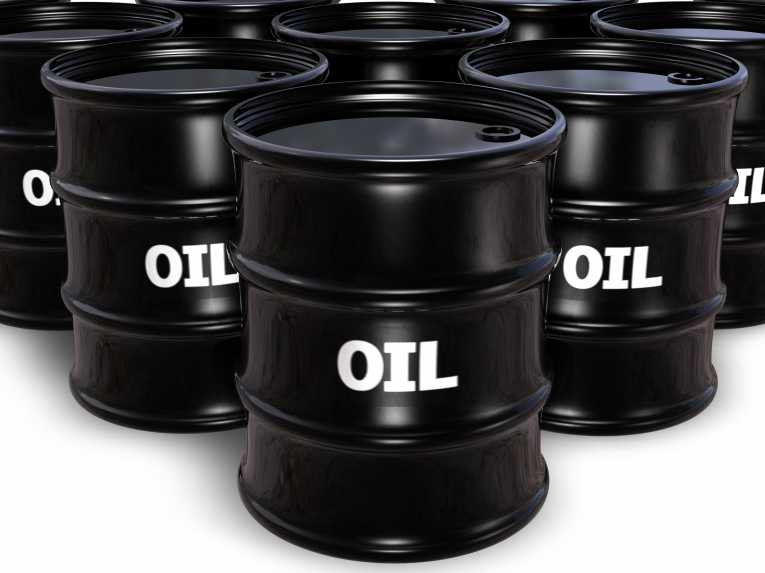
\includegraphics[scale=0.10]{./Chapter1/Figures/figure-oil.jpg}};
\node [anchor=north west] (part1text) at ([xshift=-1em,yshift=0.0em]part1label.south west) {\begin{tabular}{l}{\color{red}{资源}}:可以使机器翻译\\系统运行的“汽油”\end{tabular}};
\end{scope}
}

{
\begin{scope}[yshift=-1.0in,xshift=2.8in]
\node [] (part2label) at (0,0) {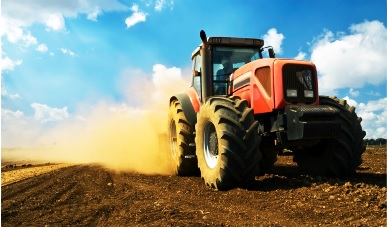
\includegraphics[scale=0.33]{./Chapter1/Figures/figure-truck.jpg}};
\node [anchor=north west] (part2text) at ([xshift=-1em,yshift=0em]part2label.south west) {\begin{tabular}{l}{\color{red}{系统}}:利用资源完成\\自动翻译的程序\end{tabular}};
\end{scope}
}

{
\draw[<-,thick] (part1label.north)..controls +(north:0.6) and +(south:0.6)..([yshift=0.2em]part1.south);
}

{
\draw[<-,thick] ([yshift=0.0em]part2label.north)..controls +(north:0.6) and +(south:0.6)..([yshift=0.2em]part2.south);
}

\end{tikzpicture}



    \caption{机器翻译系统的组成}
    \label{fig:1-2}
\end{figure}
%-------------------------------------------

\begin{itemize}
\vspace{0.5em}
\item {\small\bfnew{资源}}:如果把机器翻译系统比作一辆汽车,资源就好比是可以使汽车运行的“汽油”,它包括很多内容,如翻译规则、双(单)语数据、知识库等翻译知识,且这些“知识”都是计算机可读的。值得一提的是,如果没有翻译资源的支持,任何机器翻译系统都无法运行起来。
\vspace{0.5em}
\item {\small\bfnew{系统}}:机器翻译算法的程序实现被称作系统,也就是机器翻译研究人员开发的软件。无论是翻译规则、翻译模板还是统计模型中的参数都需要通过机器翻译系统进行读取和使用。
\vspace{0.5em}
\end{itemize}

\parinterval 构建一个强大的机器翻译系统需要“资源”和“系统”两方面共同作用。在资源方面,随着语料库语言学的发展,已经有大量的高质量的双语和单语数据(称为语料)被整理并且被数字化存储,因此可以说具备了研发机器翻译系统所需要的语料基础。特别是像英语、汉语等世界主流语种,相关语料资源已经非常丰富,这也大大加速了相关研究的进展。当然,对于一些稀缺资源语种或者特殊的领域,语料库中的语料仍然匮乏,但是这些并不影响机器翻译领域整体的发展速度。因此在现有语料库的基础上,很多研究者把精力集中在“系统”研发上。

%----------------------------------------------------------------------------------------
%    NEW SECTION
%----------------------------------------------------------------------------------------

\sectionnewpage
\section{机器翻译简史}

\parinterval 虽然翻译这个概念在人类历史中已经存在了上千年,但机器翻译发展至今只有七十余年的历史。纵观机器翻译的发展,历程曲折又耐人寻味,可以说,回顾机器翻译的历史对深入理解相关技术方法会有很好的启发,甚至对了解整个自然语言处理领域的发展也有启示作用。

%----------------------------------------------------------------------------------------
%    NEW SUB-SECTION
%----------------------------------------------------------------------------------------

\subsection{人工翻译}

\parinterval 人类形成语言文字的过程中逐渐形成了翻译的概念。一个著名的标志性证据是罗塞塔石碑(Rosetta Stone),如图\ref{fig:1-3}所示。这个石碑制作于公元前196年,据说是可供考证的最久远的记载平行文字的历史遗迹。石碑由上至下刻有同一段埃及国王诏书的三种语言版本,最上面是古埃及象形文,中间是埃及草书,最下面是古希腊文。可以明显看出石碑上中下雕刻的文字的纹理是不同的。尽管用不同的语言文字描述同一件事在今天看来很常见,但是这在生产力低下的两千年前是很罕见的。很多人认为罗塞塔石碑是标志翻译或人工翻译的一个起点。目前罗塞塔石碑保存于大英博物馆,并成为该馆最具代表性的镇馆之宝之一。

%----------------------------------------------
\begin{figure}[htp]
    \centering
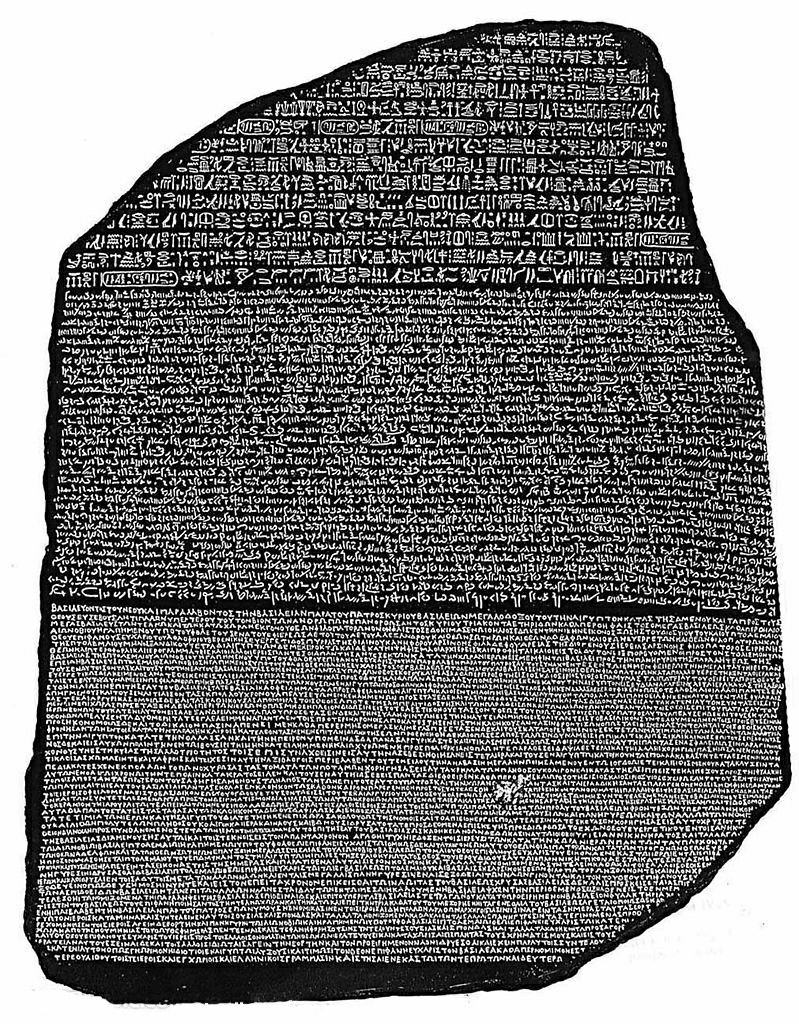
\includegraphics[scale=0.20]{./Chapter1/Figures/figure-rosetta-stone.jpg}
    \caption{罗塞塔石碑}
    \label{fig:1-3}
\end{figure}
%------------------------------------------

\parinterval 在此之后,更多的翻译工作在文化和知识传播中开展。其中一个典型代表是宗教文献的翻译。宗教是人类意识形态的一个重要载体,为了宣传教义,人们编写了大量的宗教文献。在西方,一项最早被记录的翻译活动是将旧约圣经(希伯来文及埃兰文)翻译为希腊文版本。迄今为止人类历史上翻译版本最多的书就是圣经。在中国唐代,有一位世界性的文化人物\ \dash \ 玄奘,他不仅是佛学家、旅行家,还是翻译家。玄奘西行求法归来后把全部的心血和智慧奉献给了译经事业,在助手们的帮助下,共翻译佛教经论74部,1335卷,每卷万字左右,合计1335万字,占去整个唐代译经总数的一半以上\upcite{慧立2000大慈恩寺三藏法師傳},树立了我国古代翻译思想的光辉典范。

\parinterval 翻译在人类历史长河中起到了重要的作用。一方面,由于语言文字、文化和地理位置的差异性,使得翻译成为一个重要的需求;另一方面,翻译也加速了不同文明的融会贯通,促进了世界的发展。今天,翻译已经成为重要的行业之一,包括各个高校也都设立了翻译及相关专业,相关人才不断涌现。据《2019年中国语言服务行业发展报告》\upcite{2019cns}统计:全球语言服务产值预计将首次接近500亿美元;中国涉及语言服务的在营企业360,000余家,语言服务为主营业务的在营企业近万家,总产值超过300亿元,年增长3\%以上;全国开设外语类专业的高校数量多达上千所,其中设立有翻译硕士(MTI)和翻译本科(BTI)专业的院校分别有250余所和280余所,其中仅MTI的累计招生数就高达6万余人\upcite{赵军峰2019深化改革}。当然,面对着巨大的需求,如何使用机器辅助翻译等技术手段提高人工翻译效率,也是人工翻译和机器翻译领域需要共同探索的方向。

%----------------------------------------------------------------------------------------
%    NEW SUB-SECTION
%----------------------------------------------------------------------------------------

\subsection{机器翻译的萌芽}

\parinterval 人工翻译已经存在了上千年,而机器翻译又起源于什么时候呢?机器翻译跌宕起伏的发展史可以分为萌芽期、受挫期、快速成长期和爆发期四个阶段。

\parinterval 早在17世纪,如Descartes、Leibniz、Cave\ Beck、Athanasius\ Kircher和Johann\ Joachim\ Becher等很多学者就提出采用机器词典(电子词典)来克服语言障碍的想法\upcite{knowlson1975universal},这种想法在当时是很超前的。随着语言学、计算机科学等学科的发展,在19世纪30年代使用计算模型进行自动翻译的思想开始萌芽,如当时法国科学家Georges Artsrouni就提出用机器来进行翻译的想法。只是那时依然没有合适的实现手段,所以这种想法的合理性无法被证实。

\parinterval 随着第二次世界大战爆发, 对文字进行加密和解密成为重要的军事需求,这也使得数学和密码学变得相当发达。在战争结束一年后,世界上第一台通用电子数字计算机于1946年研制成功,至此使用机器进行翻译有了真正实现的可能。

\parinterval 基于战时密码学领域与通讯领域的研究,Claude Elwood Shannon在1948年提出使用“噪声信道”描述语言的传输过程,并借用热力学中的“{\small\bfnew{熵}}\index{熵}”(Entropy)\index{Entropy}来刻画消息中的信息量\upcite{DBLP:journals/bstj/Shannon48}。次年,Shannon与Warren Weaver更是合著了著名的\emph{The Mathematical Theory of Communication}\upcite{shannon1949the},这些工作都为后期的统计机器翻译打下了理论基础。

\parinterval 1949年,Weaver撰写了一篇名为\emph{TRANSLATION}的备忘录\upcite{weaver1955translation},在这个备忘录中Weaver提出用密码学的方法解决人类语言翻译任务的想法,比如把汉语看成英语的一个加密文本,那么将汉语翻译成英语就类似于解密的过程。并且在这篇备忘录中第一次提出了机器翻译,正式开创了机器翻译的概念,这个概念一直沿用至今。虽然,在那个年代进行机器翻译的研究条件并不成熟,包括使用加密解密技术进行自动翻译的很多尝试很快也被验证是不可行的,但是这些早期的探索为后来机器翻译的发展提供了思想的火种。

%----------------------------------------------------------------------------------------
%    NEW SUB-SECTION
%----------------------------------------------------------------------------------------

\subsection{机器翻译的受挫}

\parinterval 随着电子计算机的发展,研究者开始尝试使用计算机来进行自动翻译。1954年,美国乔治敦大学在IBM公司支持下,启动了第一次真正的机器翻译实验。翻译的目标是将几个简单的俄语句子翻译成为英语,翻译系统包含6条翻译规则和250个单词。这次翻译实验中测试了50个化学文本句子,取得了初步成功。在某种意义上来说,这个实验显示了采用基于词典和翻译规则的方法可以实现机器翻译过程。虽然只是取得了初步成功,但却引起了苏联、英国和日本研究机构的机器翻译研究热,大大推动了早期机器翻译的研究进展。

\parinterval 1957年,Noam Chomsky在\emph{Syntactic Structures}中描述了转换生成语法\upcite{chomsky1957syntactic},并使用数学方法来研究自然语言,建立了包括上下文有关语法、上下文无关语法等4种类型的语法。这些工作最终为今天计算机中广泛使用的“形式语言”奠定了基础。而他的思想也深深地影响了同时期的语言学和自然语言处理领域的学者。特别的是,早期基于规则的机器翻译中也大量使用了这些思想。

\parinterval 虽然在这段时间,使用机器进行翻译的议题越加火热,但是事情并不总是一帆风顺,怀疑论者对机器翻译一直存有质疑,并很容易找出一些机器翻译无法解决的问题。自然地,人们也期望能够客观地评估一下机器翻译的可行性。当时美国基金资助组织委任自动语言处理咨询会承担了这项任务。经过近两年的调查与分析,该委员会于1966年11月公布了一个题为\emph{LANGUAGE AND MACHINES}的报告(图\ref{fig:1-4}),即ALPAC报告。该报告全面否定了机器翻译的可行性,为机器翻译的研究泼了一盆冷水。

%----------------------------------------------
\begin{figure}[htp]
    \centering
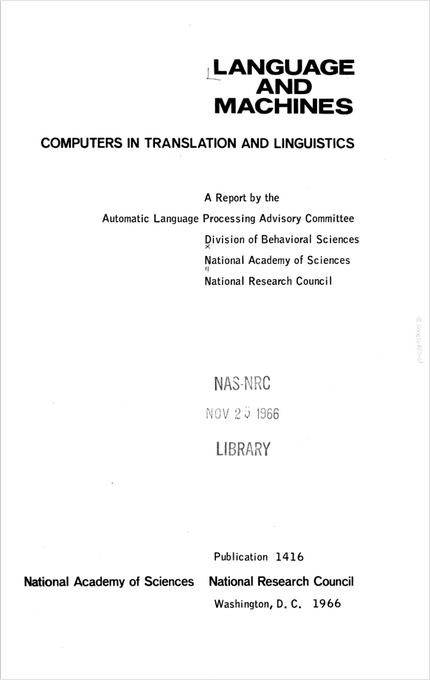
\includegraphics[scale=0.65]{./Chapter1/Figures/figure-report.jpg}
    \caption{ALPAC报告}
    \label{fig:1-4}
\end{figure}
%-------------------------------------------

\parinterval 随后美国政府终止了对机器翻译研究的支持,这导致整个产业界和学术界都开始回避机器翻译。没有了政府的支持,企业也无法进行大规模投入,机器翻译的研究就此受挫。

\parinterval 从历史上看,包括机器翻译在内,很多人工智能领域在那个年代并不受“待见”,其主要原因在于当时的技术水平还比较低,而大家又对机器翻译等技术的期望过高。最后发现,当时的机器翻译水平无法满足实际需要,因此转而排斥它。但是,也正是这一盆冷水,让研究人员可以更加冷静地思考机器翻译的发展方向,为后来的爆发蓄力。

%----------------------------------------------------------------------------------------
%    NEW SUB-SECTION
%----------------------------------------------------------------------------------------

\subsection{机器翻译的快速成长}

\parinterval 事物的发展都是螺旋式上升的,机器翻译也是一样。早期基于规则的机器翻译方法需要人来书写规则,虽然对少部分句子具有较高的翻译精度,可是对翻译现象的覆盖度有限,而且对规则或者模板中的噪声非常敏感,系统健壮性差。

\parinterval 上世纪70年代中后期,特别是80年代到90年代初,国家之间往来日益密切,而不同语言之间形成的交流障碍愈发严重,传统的人工作业方式已经远远不能满足需求。与此同时,语料库语言学的发展也为机器翻译提供了新的思路。一方面,随着传统纸质文字资料不断电子化,计算机可读的语料越来越多,这使得人们可以用计算机对语言规律进行统计分析。另一方面,随着可用数据越来越多,用数学模型描述这些数据中的规律并进行推理逐渐成为可能。这也衍生出一类数学建模方法\ \dash\ {\small\bfnew{数据驱动}}\index{数据驱动}(Data-driven)\index{Data-driven}的方法。同时这类方法也成为了随后出现的统计机器翻译的基础,比如,IBM研究人员提出的基于噪声信道模型的5种统计翻译模型就使用了这类方法\upcite{brown1990statistical,DBLP:journals/coling/BrownPPM94}。

\parinterval 基于数据驱动的方法不依赖于人书写的规则,机器翻译的建模、训练和推断都可以自动地从数据中学习。这使得整个机器翻译的范式发生了翻天覆地的变化,比如,日本学者长尾真提出的基于实例的方法\upcite{nagao1984framework,DBLP:conf/coling/SatoN90}和统计机器翻译\upcite{brown1990statistical,DBLP:journals/coling/BrownPPM94}就是在此期间兴起的。此外,这样的方法使得机器翻译系统的开发代价大大降低。

\parinterval 从上世纪90年代到本世纪初,随着语料库的完善与高性能计算机的发展,统计机器翻译很快成为了当时机器翻译研究与应用的代表性方法。一个标志性的事件是谷歌公司推出了一个在线的免费自动翻译服务,也就是大家熟知的谷歌翻译。这使得机器翻译这种“高大上”的技术快速进入人们的生活,而不再是束之高阁的科研想法。随着机器翻译不断走向实用,机器翻译的应用也越来越多,这反过来促进了机器翻译的研究进程。比如,在2005-2015年间,统计机器翻译这个主题几乎统治了ACL等自然语言处理相关方向顶级会议的论文,可见其在当时的影响力。

%----------------------------------------------------------------------------------------
%    NEW SUB-SECTION
%----------------------------------------------------------------------------------------

\subsection{机器翻译的爆发}

\parinterval 进入二十一世纪,统计机器翻译拉开了黄金发展期的序幕。在这一时期,各种基于统计机器翻译模型层出不穷,经典的基于短语的模型和基于句法的模型也先后被提出。在2013年以后,机器学习的进步带来了机器翻译技术的进一步提升。特别是基于神经网络的深度学习方法在机器视觉、语音识别中被成功应用,带来性能的飞跃式提升。很快,深度学习方法也被用于机器翻译。

\parinterval 实际上,对于机器翻译任务来说,深度学习方法被广泛使用也是一种必然,原因如下:

\begin{itemize}
\vspace{0.5em}
\item 第一,端到端学习不依赖于过多的先验假设。在统计机器翻译时代,模型设计或多或少会对翻译的过程进行假设,称为隐藏结构假设。比如基于短语的模型假设:源语言和目标语言都会被切分成短语序列,这些短语之间存在某种对齐关系。这种假设既有优点也有缺点:一方面,该假设有助于模型融入人类的先验知识,比如,统计机器翻译中一些规则的设计就借鉴了语言学的相关概念;另一方面,假设越多模型受到的限制也越多。如果假设是正确的,模型可以很好地描述问题。但如果假设错误,那么模型就可能产生偏差。深度学习不依赖于先验知识,也不需要手工设计特征,模型直接从输入和输出的映射上进行学习(端到端学习),这样也在一定程度上避免了隐藏结构假设造成的偏差。
\vspace{0.5em}
\item 第二,神经网络的连续空间模型有更强的表示能力。机器翻译中的一个基本问题是:如何表示一个句子?统计机器翻译把句子的生成过程看作是短语或者规则的推导,这本质上是一个离散空间上的符号系统。深度学习把传统的基于离散化的表示变成了连续空间的表示。比如,用实数空间的分布式表示代替了离散化的词语表示,而整个句子可以被描述为一个实数向量。这使得翻译问题可以在连续空间上描述,进而大大缓解了传统离散空间模型维度灾难等问题。更重要的是,连续空间模型可以用梯度下降等方法进行优化,具有很好的数学性质并且易于实现。
\vspace{0.5em}
\item 第三,深度网络学习算法的发展和{\small\bfnew{图形处理单元}}(Graphics Processing Unit\index{Graphics Processing Unit},GPU)等并行计算设备为训练神经网络提供了可能。早期的基于神经网络的方法一直没有在机器翻译甚至自然语言处理领域得到大规模应用,其中一个重要的原因是这类方法需要大量的浮点运算,但是以前计算机的计算能力无法达到这个要求。随着GPU等并行计算设备的进步,训练大规模神经网络也变为了可能。现在已经可以在几亿、几十亿,甚至上百亿句对上训练机器翻译系统,系统研发的周期越来越短,进展日新月异。
\vspace{0.5em}
\end{itemize}

\parinterval 今天,神经机器翻译已经成为新的范式,与统计机器翻译一同推动了机器翻译技术与应用产品的发展。比如,从世界上著名的机器翻译比赛WMT和CCMT中就可以看出这个趋势。如图\ref{fig:1-5}所示,其中左图是WMT\ 19国际机器翻译比赛的参赛队伍的截图,这些参赛队伍基本上都在使用深度学习完成机器翻译的建模。而在WMT\ 19各个项目的夺冠系统中(\ref{fig:1-5}右图),神经机器翻译也占据了主导地位。

%----------------------------------------------
\begin{figure}[htp]
    \centering
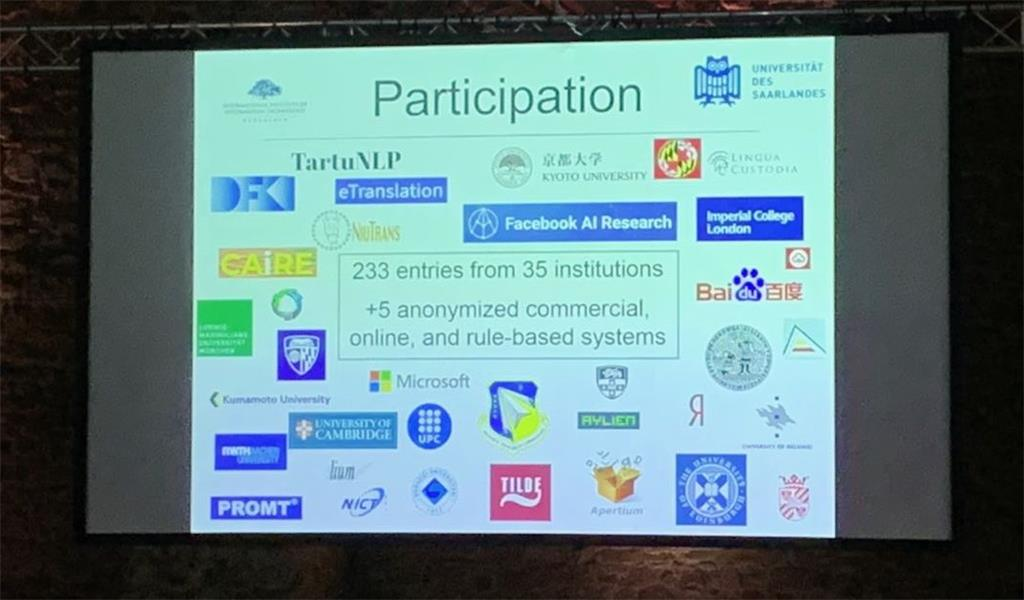
\includegraphics[scale=0.3]{./Chapter1/Figures/figure-wmt-participation.jpg}
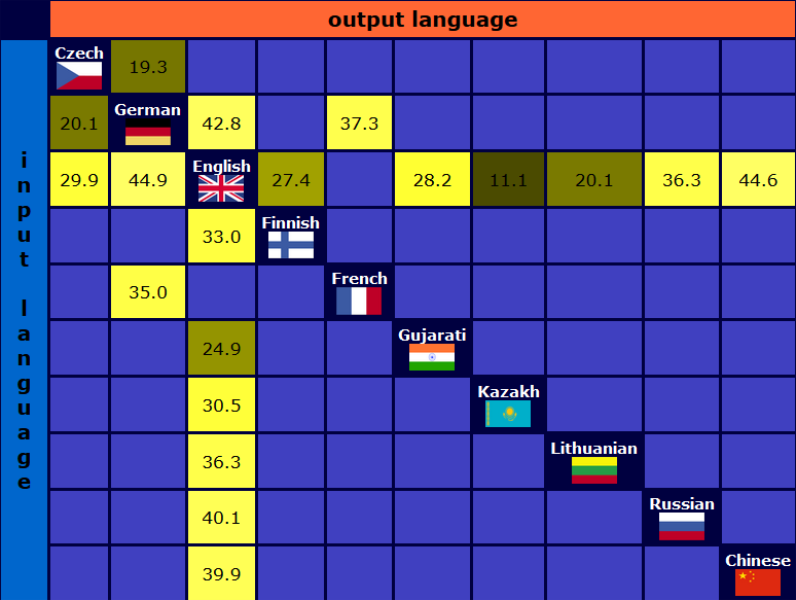
\includegraphics[scale=0.3]{./Chapter1/Figures/figure-wmt-bestresults.jpg}
\setlength{\belowcaptionskip}{-1.5em}
    \caption{WMT\ 19国际机器翻译大赛(左:WMT\ 19参赛队伍;右:WMT\ 19各项目的最高分数)}
    \label{fig:1-5}
\end{figure}
%-------------------------------------------

\parinterval 值得一提的是,近些年神经机器翻译的快速发展也得益于产业界的关注。各大互联网企业和机器翻译技术研发机构都对神经机器翻译的模型和实践方法给予了很大贡献。很多企业凭借自身人才和基础设施方面的优势,先后推出了以神经机器翻译为内核的产品及服务,相关技术方法已经在大规模应用中得到验证,大大推动了机器翻译的产业化进程,而且这种趋势在不断加强,机器翻译的前景也更加宽广。

%----------------------------------------------------------------------------------------
%    NEW SECTION
%----------------------------------------------------------------------------------------

\sectionnewpage
\section{机器翻译现状及挑战}
%%%%%%%%%%%%%%%%%%%%%%%%%%%%%%%%%%%%%%%%%%%%%%%%%%%%%%%%%%%%%%%%%%%%%%%%%%%%
\parinterval 机器翻译技术发展到今天已经过无数次迭代,技术范式也经过若干次更替,近些年机器翻译的应用也如雨后春笋相继浮现。今天的机器翻译的质量究竟如何呢?乐观地说,在很多特定的条件下,机器翻译的译文结果是非常不错的,甚至可以接近人工翻译的结果。然而,在开放式翻译任务中,机器翻译的结果还并不完美。更严格来说,机器翻译的质量远没有达到人们所期望的程度。对于有些人提到的“机器翻译将代替人工翻译”也并不是事实。比如,在高精度同声传译任务中,机器翻译仍需要更多打磨;再比如,针对于小说的翻译,机器翻译还无法做到与人工翻译媲美;甚至有人尝试用机器翻译系统翻译中国古代诗词,这里更多的是娱乐的味道。但是毫无疑问的是,机器翻译可以帮助人类,甚至有朝一日可以代替一些低端的人工翻译工作。

\parinterval 图\ref{fig:1-6}展示了机器翻译和人工翻译质量的一个对比结果。在汉语到英语的新闻翻译任务中,如果对译文进行人工评价(五分制),那么机器翻译的译文得分为3.9分,人工译文得分为4.7分(人的翻译也不是完美的)。可见,在这个任务中机器翻译表现不错,但是与人还有一定差距。如果换一种方式评价,把人的译文作为参考答案,用机器翻译的译文与其进行比对(百分制),会发现机器翻译的得分只有47分。当然,这个结果并不是说机器翻译的译文质量很差,它更多的是表明机器翻译系统可以生成一些与人工翻译不同的译文,机器翻译也具有一定的创造性。这也类似于,很多围棋选手都想向AlphaGo学习,因为智能围棋系统也可以走出一些人类从未走过的妙招。

%----------------------------------------------
\begin{figure}[htp]
   \centering

\definecolor{ublue}{rgb}{0.152,0.250,0.545}
\definecolor{ugreen}{rgb}{0,0.5,0}


%%% outline
%-------------------------------------------------------------------------

{
\begin{tikzpicture}
\node [anchor=south west, fill=blue!70, minimum width=1.1cm, minimum height=2.3cm] (mt) at (1,0) {{\color{white} {\small\sffamily\bfseries{机器}}}};
\node [anchor=south west, fill=red!70, minimum width=1.1cm, minimum height=2.7cm] (human) at ([xshift=0.5cm]mt.south east) {{\color{white} {\small\sffamily\bfseries{人}}}};
\node [anchor=south] (mtscore) at (mt.north) {3.9};
\node [anchor=south] (humanscore) at (human.north) {4.7};
\draw [->,very thick] ([xshift=-0.5cm]mt.south west) -- ([xshift=0.5cm]human.south east);
\draw [->,very thick] ([xshift=-0.5cm]mt.south west) -- ([xshift=-0.5cm,yshift=3.2cm]mt.south west);
\node [anchor=north west] (x1) at ([xshift=0.0cm]human.south east) {\footnotesize{评价对象}};
\node [anchor=north east] (y1) at ([xshift=-0.5cm,yshift=3.2cm]mt.south west) {\footnotesize{打分}};
\node [anchor=north] (y2) at ([yshift=-0cm]y1.south) {\footnotesize{(分)}};

\node [anchor=south west, fill=blue!70, minimum width=1.1cm, minimum height=1.5cm] (mt1) at ([xshift=16.0em,yshift=-3.0em]mt.east) {{\color{white} {\small\sffamily\bfseries{机器}}}};
\node [anchor=south west, fill=red!70, minimum width=1.1cm, minimum height=2.7cm] (human1) at ([xshift=0.5cm]mt1.south east) {{\color{white} {\small\sffamily\bfseries{人}}}};
\node [anchor=south] (mtscore1) at (mt1.north) {47};
\node [anchor=south] (humanscore1) at (human1.north) {100};
\draw [->,very thick] ([xshift=-0.5cm]mt1.south west) -- ([xshift=0.5cm]human1.south east);
\draw [->,very thick] ([xshift=-0.5cm]mt1.south west) -- ([xshift=-0.5cm,yshift=3.2cm]mt1.south west);
\node [anchor=north west] (x1) at ([xshift=0.0cm]human1.south east) {\footnotesize{评价对象}};
\node [anchor=north east] (y1) at ([xshift=-0.5cm,yshift=3.2cm]mt1.south west) {\footnotesize{打分}};
\node [anchor=north] (y2) at ([yshift=-0cm]y1.south) {\footnotesize{(分)}};

\node[anchor=south](footname1) at ([xshift=2.1em,yshift=-2.0em]mt.south){\footnotesize{人工评价(五分制)}};
\node[anchor=south](footname2) at ([xshift=2.1em,yshift=-2.0em]mt1.south){\footnotesize{自动评价(百分制)}};
\end{tikzpicture}

}






%---------------------------------------------------------------------




\setlength{\belowcaptionskip}{-0.5em}
    \caption{机器翻译与人工翻译性能对比(汉英新闻领域翻译)}
    \label{fig:1-6}
\end{figure}
%-------------------------------------------

\parinterval 图\ref{fig:1-7}展示了一个真实的汉语到英语翻译实例。对比发现,机器翻译与人工翻译还是存在差距的,特别是在翻译一些具有感情色彩的词语时,机器翻译的译文缺一些味道。那么,机器翻译一点用都没有吗?显然不是。实际上,如果考虑翻译速度与翻译代价,机器翻译的价值是无可比拟的。还是同一个例子,翻译一篇短文如果人工翻译需要30分钟甚至更长时间,那么机器翻译仅仅需要两秒,换种情况思考,如果有100万篇这样的文档,其人工翻译的成本根本无法想象,消耗的时间更是难以计算,而计算机集群仅仅需要一天,而且只有电力的消耗。

%----------------------------------------------
\begin{figure}[htp]
    \centering
\definecolor{ublue}{rgb}{0.152,0.250,0.545}
\definecolor{ugreen}{rgb}{0,0.5,0}

%%% outline
%-------------------------------------------------------------------------
\begin{tikzpicture}
%第一段----------------------------------------------
%原文-------------
\node [pos=0.4,left,xshift=-0.4em,yshift=2.0em] (original1) {\scriptsize{源\ \ 语\ \ 言:从前有一个小岛,上面住着快乐、悲哀、知识和爱,还有其他各种情感。一天,情感们得知}};
\node [anchor=north west] (original1-1) at ([xshift=3.5em,yshift=0.3em]original1.south west)  {\scriptsize{小岛快要下沉了。于是,大家都准备船只,离开小岛,只有爱决定留下来,她想坚持到最后}};
\node [anchor=north west] (original1-2) at ([yshift=0.3em]original1-1.south west)  {\scriptsize{一刻。过了几天,小岛真的要下沉了,爱想请人帮忙。}};
%机器翻译--------------
\node [anchor=north west] (mt1) at ([xshift=-3.5em,yshift=0.3em]original1-2.south west) {\scriptsize{机器翻译:Once upon a time there was an island {\color{red}\underline{on which}} lived happiness,sorrow,knowledge,love and other}};

\node [anchor=north west] (mt1-1) at ([xshift=3.5em,yshift=0.4em]mt1.south west) {\scriptsize{emotions. One day, {\color{red}\underline{the}} emotions learned that the island was going to sink.As a result,everyone pre}};

\node [anchor=north west] (mt1-2) at ([yshift=0.4em]mt1-1.south west) {\scriptsize{-pared the boat and {\color{red}\underline{left the island.}} Only Love decided to stay.She {\color{red}\underline{ wanted to stick}} to it until the last}};

\node [anchor=north west] (mt1-3) at ([yshift=0.4em]mt1-2.south west) {\scriptsize{moment. After a few days, the island was really going to sink and love {\color{red}\underline{ wanted help.}}}};
%人工翻译---------------
\node [anchor=north west] (ht1) at ([xshift=-3.5em,yshift=0.4em]mt1-3.south west) {\scriptsize{人工翻译:Once upon a time, there was a small island {\color{red}\underline{where}} lived all kinds of emotions like JOY,SADNESS,}};

\node [anchor=north west] (ht1-1) at ([xshift=3.5em,yshift=0.4em]ht1.south west) {\scriptsize{KNOWLEDGE, and LOVE.One day, {\color{red}\underline{these}} emotions found that the island was sinking, so one by}};

\node [anchor=north west] (ht1-2) at ([yshift=0.4em]ht1-1.south west) {\scriptsize{one they prepared the boat and {\color{red}\underline{planned to leave.}} None but LOVE chose to stay there. She {\color{red}\underline{was deter}}}};

\node [anchor=north west] (ht1-3) at ([yshift=0.4em]ht1-2.south west) {\scriptsize{{\color{red}\underline{-mined to}} persist till the last moment.A few days later, almost the whole island sunk into the sea,}};

\node [anchor=north west] (ht1-4) at ([yshift=0.4em]ht1-3.south west) {\scriptsize{and LOVE had to {\color{red}\underline{seek for help.}}}};

\begin{pgfonlayer}{background}
{
\node[rectangle,draw=ublue, inner sep=0mm] [fit =(original1)(ht1)(mt1)(ht1-4)] {};
}
\end{pgfonlayer}


\end{tikzpicture}





    \caption{机器翻译与人工翻译结果对比实例}
    \label{fig:1-7}
\end{figure}
%-------------------------------------------

\parinterval 虽然机器翻译有上述优点,但仍然面临一些挑战:

\begin{itemize}
\vspace{0.5em}
\item {\small\bfnew{自然语言翻译问题的复杂性极高}}。自然语言具有高度的概括性、灵活性、多样性,这些都很难用几个简单的模型和算法进行描述。因此,翻译问题的数学建模和计算机程序实现难度很大。虽然近几年AlphaGo等人工智能系统在围棋等领域取得了令人瞩目的成绩,但是,相比翻译来说,围棋等棋类任务仍然“简单”。正如不同人对同一句话的理解不尽相同,一个句子往往不存在绝对的标准译文,其潜在的译文几乎是不可穷尽的。甚至人类译员在翻译一个句子、一个单词的时候,都要考虑整个篇章的上下文语境。这些难点都不是传统棋类任务所具有的。
\vspace{0.5em}
\item {\small\bfnew{计算机的“理解”与人类的“理解”存在鸿沟}}。人类一直希望把自己翻译时所使用的知识描述出来,并用计算机程序进行实现,例如早期基于规则的机器翻译方法就源自这个思想。但是,经过实践发现,人和计算机在“理解”自然语言上存在着明显差异。首先,人类的语言能力是经过长时间在多种外部环境因素共同作用下形成的,这种能力很难用计算机准确地刻画。况且人类的语言知识本身就很难描述,更不用说让计算机来理解;其次,人和机器翻译系统理解语言的目的不一样。人理解和使用语言是为了进行生活和工作,而机器翻译系统更多的是为了对某些数学上定义的目标函数进行优化。也就是说,机器翻译系统关注的是翻译这个单一目标,而并不是像人一样进行复杂的活动;此外,人和计算机的运行方式有着本质区别。人类语言能力的生物学机理与机器翻译系统所使用的计算模型本质上是不同的,机器翻译系统使用的是其自身能够理解的“知识”,比如,统计学上的词语表示。这种“知识”并不需要人来理解,当然从系统开发的角度,计算机也并不需要理解人是如何思考的。
\vspace{0.5em}
\item {\small\bfnew{单一的方法无法解决多样的翻译问题}}。首先,语种的多样性会导致任意两种语言之间的翻译实际上都是不同的翻译任务。比如,世界上存在的语言多达几千种,如果选择任意两种语言进行互译就会产生上百万种翻译方向。虽然已经有研究者尝试用同一个框架甚至同一个翻译系统进行全语种的翻译,但是这类系统离真正可用还有很远的距离;其次,不同的领域,不同的应用场景对翻译也有不同的需求。比如,文学作品的翻译和新闻的翻译就有不同、口译和笔译也有不同,类似的情况不胜枚举。以上这些都增加了计算机对翻译进行建模的难度;再次,对于机器翻译来说,充足的高质量数据是必要的,但是不同语种、不同领域、不同应用场景所拥有的数据量有明显差异,很多语种甚至几乎没有可用的数据,这时开发机器翻译系统的难度可想而知。值得注意的是,现在的机器翻译还无法像人类一样在学习少量样例的情况下进行举一反三,因此数据稀缺情况下的机器翻译也给研究者带来了很大的挑战。
\vspace{0.5em}
\end{itemize}

\parinterval 显然,实现机器翻译并不简单,甚至有人把机器翻译看作是实现人工智能的终极目标。幸运的是,今天的机器翻译无论从技术方法上还是从应用上都有了巨大的飞跃,很多问题在不断被求解。如果读者看到过十年前机器翻译的结果,再对比今天的结果,一定会感叹翻译质量的今非昔比,很多译文已经非常准确且流畅。从当今机器翻译的前沿技术看,近三十年机器翻译的进步更多得益于基于数据驱动方法和统计建模方法的使用。特别是近些年深度学习等基于表示学习的端到端方法使得机器翻译的水平达到了新高度。因此,本书将会对基于统计建模和深度学习方法的机器翻译模型、方法和系统实现进行全面介绍和分析,希望这些论述可以对相关内容的学习和科研工作提供参考。

%----------------------------------------------------------------------------------------
%    NEW SECTION
%----------------------------------------------------------------------------------------

\sectionnewpage
\section{基于规则的方法}\label{section-1.4}
%%%%%%%%%%%%%%%%%%%%%%%%%%%%%%%%%%%%%%%%%%%%%%%%%%%%%%%%%%%%%%%%%%%%%%%%%%%%
\parinterval 机器翻译技术大体上可以分为两种方法,分别为基于规则的机器翻译方法以及数据驱动的机器翻译方法。进一步,数据驱动的机器翻译方法又可以分为统计机器翻译方法以及神经机器翻译方法。第一代机器翻译技术是主要使用基于规则的机器翻译方法,其主要思想是通过形式文法定义的规则引入源语言和目标语言中的语言学知识。此类方法在机器翻译技术诞生之初就被人所关注,特别是在上世纪70年代,以基于规则方法为代表的专家系统是人工智能中最具代表性的研究领域。甚至到了统计机器翻译时代,很多系统中也大量地使用了基于规则的翻译知识表达形式。

\parinterval 早期,基于规则的机器翻译大多依赖人工定义及书写的规则。主要有两类方法\upcite{nirenburg1989knowledge,hutchins1986machine,zarechnak1979history}:一类是基于转换规则的机器翻译方法,简称转换法。另一类是基于中间语言的方法。它们都以词典和人工书写的规则库作为翻译知识,用一系列规则的组合完成翻译。

%----------------------------------------------------------------------------------------
%    NEW SUB-SECTION
%----------------------------------------------------------------------------------------

\subsection{规则的定义}

\parinterval 规则就像语言中的“If-then”语句,如果满足条件,则执行相应的语义动作。比如,可以将待翻译句子中的某个词,使用目标语言单词进行替换,但是这种替换并非随意的,而是在语言学知识的指导下进行的。

%----------------------------------------------
\begin{figure}[htp]
    \centering
\definecolor{ublue}{rgb}{0.152,0.250,0.545}
\definecolor{ugreen}{rgb}{0,0.5,0}


%%% outline
%-------------------------------------------------------------------------

\begin{tikzpicture}
\begin{scope}
{
{\footnotesize
\node [anchor=north west] (rule1) at (0,0) {\textbf{1: If} 源=我, \textbf{then} 译=\ I};
\node [anchor=north west] (rule2) at ([yshift=0.1em]rule1.south west) {\textbf{2: If} 源=你, \textbf{then} 译=\ you};
\node [anchor=north west] (rule3) at ([yshift=0.1em]rule2.south west) {\textbf{3: If} 源=感到\ 满意,};
\node [anchor=north west] (rule3part2) at ([yshift=0.5em]rule3.south west) {\textbf{\hspace{0.95em} then} 译=\ be satisfied with};
\node [anchor=north west] (rule4) at ([yshift=0.1em]rule3part2.south west) {\textbf{4: If} 源=对 ... 动词[表态度]};
\node [anchor=north west] (rule4part2) at ([yshift=0.5em]rule4.south west) {\textbf{\hspace{0.95em} then} 调序[动词 + 对象]};
\node [anchor=north west] (rule5) at ([yshift=0.1em]rule4part2.south west) {\textbf{5: If} 译文主语是\ I};
\node [anchor=north west] (rule5part2) at ([yshift=0.5em]rule5.south west) {\textbf{\hspace{0.95em} then} be动词为\ am/was};
\node [anchor=north west] (rule6) at ([yshift=0.1em]rule5part2.south west) {\textbf{6: If} 源语言是主谓结构};
\node [anchor=north west] (rule6part2) at ([yshift=0.5em]rule6.south west) {\textbf{\hspace{0.95em} then} 译文为主谓结构};
\node [anchor=south west] (rulebaselabel) at (rule1.north west) {{\color{ublue} 资源:规则库}};
}

\begin{pgfonlayer}{background}
{
  \node[rectangle,draw=ublue, thick,inner sep=0mm] [fit = (rule1) (rule2) (rule3) (rule3part2) (rule4) (rule4part2) (rule5) (rule5part2) (rule6) (rule6part2) (rulebaselabel)] {};
}
\end{pgfonlayer}
}

\end{scope}

\begin{scope}[xshift=2.3in]
{\footnotesize
\node [anchor=north west,inner sep=1mm] (w1) at (0,0em) {我};
\node [anchor=north west,inner sep=1mm] (w2) at ([xshift=0.3em]w1.north east) {对};
\node [anchor=north west,inner sep=1mm] (w3) at ([xshift=0.3em]w2.north east) {你};
\node [anchor=north west,inner sep=1mm] (w4) at ([xshift=0.3em]w3.north east) {感到};
\node [anchor=north west,inner sep=1mm] (w5) at ([xshift=0.3em]w4.north east) {满意};
}
\end{scope}

{\footnotesize
\node [anchor=north,inner sep=1mm] (t1) at ([yshift=-0.6em]w1.south) {I};
\draw[->,thick,ublue] (w1.south)--(t1.north);
}

{\footnotesize
\node [anchor=north,inner sep=1mm] (t3) at ([yshift=-0.6em]w3.south) {you};
\draw[->,thick,ublue] (w3.south)--(t3.north);
}

{\footnotesize
\draw[-] ([yshift=0.2em]w4.south west)--([yshift=0.2em]w5.south east);
\node [anchor=north,inner sep=1mm] (t45) at ([yshift=-2em]w5.south) {be satisfied with};
\draw[->,thick,ublue] ([yshift=0.1em]w4.south east)..controls +(south:0.6) and +(north:0.6)..(t45.north);
}

{\footnotesize
\node [anchor=north west,inner sep=1mm] (t35) at ([yshift=-3.0em,xshift=-1em]t3.south) {be satisfied with you};
\draw[->,thick,ublue] (t3.south)..controls +(south:1.3) and +(north:0.9)..([xshift=-1em,yshift=-0.2em]t35.north east);
\draw[->,thick,ublue] (t45.south)..controls +(south:0.7) and +(north:0.5)..([xshift=3em,yshift=-0.2em]t35.north west);
}

{\footnotesize
\node [anchor=north west,inner sep=1mm] (t15) at ([yshift=-1.5em,xshift=-2em]t35.south west) {I be satisfied with you};
\draw[->,thick,ublue] (t35.south)..controls +(south:0.5) and +(north:0.5)..([xshift=-5em]t15.north east);
\draw[->,thick,ublue] (t1.south)..controls +(south:1.5) and +(north:1.5)..([xshift=0.5em]t15.north west);
}


{\footnotesize
\node [anchor=north west,inner sep=1mm] (t15final) at ([yshift=-1.5em]t15.south west) {I am satisfied with you};
\node [draw,circle,thick,dotted,ublue,minimum width=1.3em] (be1) at ([xshift=1.35em,yshift=0.1em]t15.west) {};
\draw[->,thick,ublue] ([xshift=-0em]be1.south)..controls +(south:0.3) and +(north:0.4)..([xshift=1.6em,yshift=-0.2em]t15final.north west);
}
{
\draw[->,dotted,thick,red] ([xshift=-0.2em]rule5part2.east)..controls +(east:1.5) and +( west:1.5)..(t15final.west) node[pos=0.9,below,xshift=0.3em,yshift=0.0em] (applyr6) {\color{red}{\tiny\sffamily\bfseries{规则5}}};
}

\end{tikzpicture}
%---------------------------------------------------------------------



    \caption{基于规则的机器翻译的示例图(左:规则库;右:规则匹配结果)}
    \label{fig:1-8}
\end{figure}
%-------------------------------------------

\parinterval 图\ref{fig:1-8}展示了一个使用转换法进行翻译的实例。这里,利用一个简单的汉译英规则库完成对句子“我对你感到满意”的翻译。当翻译“我”时,从规则库中找到规则1,该规则表示遇到单词“我”就翻译为“I”;类似地,也可以从规则库中找到规则4,该规则表示翻译调序,即将单词“you”放到“be satisfied with”后面。这种通过规则表示单词之间对应关系的方式,也为统计机器翻译方法提供了思路。如统计机器翻译中,基于短语的翻译模型使用短语对对源语言进行替换,详细描述可以参考{\chapterseven}。

\parinterval 在上述例子中可以发现,规则不仅仅可以翻译句子之间单词的对应,如规则1,还可以表示句法甚至语法之间的对应,如规则6。因此基于规则的方法可以分成多个层次,如图\ref{fig:1-9}所示。图中不同的层次表示采用不同的知识来书写规则,进而完成机器翻译过程。对于翻译问题,可以构建不同层次的基于规则的机器翻译系统。这里包括四个层次,分别为:词汇转换、句法转换、语义转换和中间语言层。其中,上层可以继承下层的翻译知识,比如说句法转换层会利用词汇转换层知识。早期基于规则的方法属于词汇转换层。

%----------------------------------------------
\begin{figure}[htp]
    \centering
%%%------------------------------------------------------------------------------------------------------------
%%%  短语系统的架构
\begin{center}
\begin{tikzpicture}
\begin{scope}

\tikzstyle{node1} = [minimum width=7em,minimum height=1.7em,draw,thick,fill=red!20,rounded corners=0.3em];
\tikzstyle{node2} = [minimum width=7em,minimum height=2.5em,draw,thick,fill=blue!20,rounded corners=0.3em];
\tikzstyle{node3} = [minimum width=7em,minimum height=2.5em,draw,thick,fill=green!20,rounded corners=0.3em];
\tikzstyle{node4} = [minimum width=7em,minimum height=1.7em,draw,thick,fill=orange!20,rounded corners=0.3em];
\tikzstyle{node5} = [minimum width=4.5em,minimum height=1.7em,thick,dashed];

\node [node1,anchor=south west] (s1) at (0,0) {{ \small{源语言词串}}};
\node [node2,anchor=south] (s2) at ([xshift=2.5em,yshift=2em]s1.north) {};
\node [anchor=north,minimum height=1.2em] (s21) at (s2.north) {{ \small{源语言}}};
\node [anchor=south,minimum height=1.2em] (s22) at (s2.south) {{ \small{句法结构}}};
\node [node3,anchor=south] (s3) at ([xshift=2.5em,yshift=2em]s2.north) {};
\node [anchor=north,minimum height=1.2em] (s31) at (s3.north) {{ \small{源语言}}};
\node [anchor=south,minimum height=1.2em] (s32) at (s3.south) {{ \small{语义结构}}};
\node [node4,anchor=south] (s4) at ([xshift=6em,yshift=2em]s3.north) {{ \small{中间语言(知识表示)}}};

\node [node3,anchor=north] (t1) at ([xshift=6em,yshift=-2em]s4.south) {};
\node [anchor=north,minimum height=1.2em] (t11) at (t1.north) {{ \small{目标语言}}};
\node [anchor=south,minimum height=1.2em] (t12) at (t1.south) {{ \small{语义结构}}};
\node [node2,anchor=north] (t2) at ([xshift=2.5em,yshift=-2em]t1.south) {};
\node [anchor=north,minimum height=1.2em] (t21) at (t2.north) {{ \small{目标语言}}};
\node [anchor=south,minimum height=1.2em] (t22) at (t2.south) {{ \small{句法结构}}};
\node [node1,anchor=north] (t3) at ([xshift=2.5em,yshift=-2em]t2.south) {{ \small{目标语言词串}}};

\node [anchor=north] (l1) at ([yshift=-2em]s4.south) {{ \small{语义\ 转换}}};
\node [anchor=north] (l2) at ([yshift=-3em]l1.south) {{ \small{句法\ 转换}}};
\node [anchor=north] (l3) at ([yshift=-2.5em]l2.south) {{ \small{词汇\ 转换}}};

\node [node5,anchor=north,draw] (st1) at ([xshift=-3em,yshift=-0.5em]l3.south) {{ \small{分析部分}}};
\node [node5,anchor=north,draw] (st2) at ([xshift=3em,yshift=-0.5em]l3.south) {{ \small{生成部分}}};

\draw [->,thick] (s1.north) -- ([xshift=-0.6em]s2.south);
\draw [->,thick] ([xshift=0.6em]s2.north) -- (s3.south);
\draw [->,thick] ([xshift=1.2em]s3.north) -- ([xshift=-2.7em]s4.south);
\draw [->,thick] ([xshift=2.7em]s4.south) -- ([xshift=-1.2em]t1.north);
\draw [->,thick] (t1.south) -- ([xshift=-0.6em]t2.north);
\draw [->,thick] ([xshift=0.6em]t2.south) -- (t3.north);
\draw [->,thick] (s3.east) -- (t1.west);
\draw [->,thick] (s2.east) -- (t2.west);
\draw [->,thick] (s1.east) -- (t3.west);

\draw [-] ([xshift=0.1em]s4.south) -- ([xshift=0.1em,yshift=-14em]s4.south);


\end{scope}
\end{tikzpicture}
\end{center}
    \caption{基于规则的机器翻译方法的四个层次\upcite{冯志伟2004机器翻译研究}}
\setlength{\belowcaptionskip}{-1.5em}
    \label{fig:1-9}
\end{figure}
%-------------------------------------------

%----------------------------------------------------------------------------------------
%    NEW SUB-SECTION
%----------------------------------------------------------------------------------------

\subsection{转换法}

\parinterval 通常一个典型的{\small\bfnew{基于转换规则的机器翻译}}\index{基于转换规则的机器翻译}(Transfer-based Translation)\index{Transfer-based Translation}的过程可以被视为“独立分析-相关转换-独立生成”的过程\upcite{parsing2009speech}。如图\ref{fig:1-10}所示,这些过程可以分成六个步骤,其中每一个步骤都是通过相应的翻译规则来完成。比如,第一个步骤中需要构建源语言词法分析规则,第二个步骤中需要构建源语言句法分析规则,第三个和第四个步骤中需要构建转换规则,其中包括源语言-目标语言单词和结构转换规则等等。

%----------------------------------------------
\begin{figure}[htp]
    \centering
%%%------------------------------------------------------------------------------------------------------------
%%%  短语系统的架构
\begin{center}
\begin{tikzpicture}
\begin{scope}

\tikzstyle{datanode} = [minimum width=7em,minimum height=1.7em,thick,draw,fill=red!20,rounded corners=0.3em];
\tikzstyle{modelnode} = [minimum width=7em,minimum height=1.7em,thick,draw,fill=blue!20,rounded corners=0.3em];
\tikzstyle{decodingnode} = [minimum width=7em,minimum height=1.7em,thick,draw,fill=green!20,rounded corners=0.3em];

\node [datanode,anchor=north west,minimum height=1.7em,minimum width=8em] (s1) at (0,0) {{ \small{源文句子}}};
\node [modelnode,anchor=north,minimum height=1.7em,minimum width=8em] (s2) at ([yshift=-1.5em]s1.south) {{ \small{源语词法分析}}};
\node [datanode,anchor=north,minimum height=1.7em,minimum width=8em] (s3) at ([yshift=-1.5em]s2.south) {{ \small{源文词串}}};
\node [modelnode,anchor=north,minimum height=1.7em,minimum width=8em] (s4) at ([yshift=-1.5em]s3.south) {{ \small{源语句法分析}}};
\node [datanode,anchor=north,minimum height=1.7em,minimum width=8em] (s5) at ([yshift=-1.5em]s4.south) {{ \small{源文结构}}};

\node [datanode,anchor=west,minimum height=1.7em,minimum width=8em] (t1) at ([xshift=20em]s1.east) {{ \small{译文句子}}};
\node [modelnode,anchor=north,minimum height=1.7em,minimum width=8em] (t2) at ([yshift=-1.5em]t1.south) {{ \small{目标语词法生成}}};
\node [datanode,anchor=north,minimum height=1.7em,minimum width=8em] (t3) at ([yshift=-1.5em]t2.south) {{ \small{译文词串}}};
\node [modelnode,anchor=north,minimum height=1.7em,minimum width=8em] (t4) at ([yshift=-1.5em]t3.south) {{ \small{目标语句法生成}}};
\node [datanode,anchor=north,minimum height=1.7em,minimum width=8em] (t5) at ([yshift=-1.5em]t4.south) {{ \small{译文结构}}};

\node [decodingnode,anchor=west,minimum height=1.7em,minimum width=13em,inner sep=3pt] (st1) at ([xshift=3.5em,yshift=0.85em]s5.east) {{ \small{源语-目标语单词转换}}};
\node [decodingnode,anchor=north,minimum height=1.7em,minimum width=13em,inner sep=3pt] (st2) at ([yshift=0.05em]st1.south) {{ \small{源语-目标语结构转换}}};

\draw [->,very thick] (s1.south) -- (s2.north);
\draw [->,very thick] (s2.south) -- (s3.north);
\draw [->,very thick] (s3.south) -- (s4.north);
\draw [->,very thick] (s4.south) -- (s5.north);
\draw [->,very thick] (s5.east) -- (st1.south west);
\draw [->,very thick] (st1.south east) -- (t5.west);
\draw [->,very thick] (t5.north) -- (t4.south);
\draw [->,very thick] (t4.north) -- (t3.south);
\draw [->,very thick] (t3.north) -- (t2.south);
\draw [->,very thick] (t2.north) -- (t1.south);

\end{scope}
\end{tikzpicture}
\end{center}
    \caption{基于转换规则的机器翻译的过程}
    \label{fig:1-10}
\end{figure}
%-------------------------------------------

\parinterval 转换法的目标就是使用规则定义的词法和句法,将源语言句子分解成为一个蕴含语言学标志的结构。如一个汉语句子“她把一束花放在桌上。”,经过词法和句法分析之后可以被表示成如图\ref{fig:1-11} 所示的结构,这个结构就是图\ref{fig:1-10}中的源文结构。这种使用语言学提取句子结构化表示,并使用某种规则匹配源语言结构和目标语言结构的方式也为{\chaptereight}将要介绍的基于语言学句法的模型提供了思路。

%----------------------------------------------
\begin{figure}[htp]
    \centering
%------------------------------------------------------------------------------------------------------------
%%%  句法树(层次短语)
\begin{tikzpicture}
{\small
\begin{scope}[sibling distance=25pt, level distance = 25pt]
{\scriptsize
\Tree[.\node(r){IP};
        [.\node(n11){NP}; [.\node(n21){PN};  [.\node(l1){她};]]]
        [.\node(n12){VP}; 
            [.\node(n22){BA}; \node(l2){把}; ]
            [.\node(n23){IP};
                [. \node(n31){NP}; 
                    [. \node(n41){QP}; 
                        [. \node(n51){CD};  \node(l3){一};]
                        [. \node(n52){CLP};  [.\node(n61){M};  [.\node(l4){束};]]]
                    ]
                    [. \node(n42){NP};  [.\node(n53){NN};  [.\node(l5){花};]]]
                ]
                [. \node(n32){VP}; 
                    [. \node(n43){VV};  \node(l6){放在};]
                    [. \node(n44){LCP};
                        [. \node(n54){NP};  [.\node(n62){NN};  [.\node(l7){桌};]]] 
                        [. \node(n55){LC};  \node(l8){上};]
                    ]
                ]
            ]
        ]
        [.\node(n13){PU};  \node(l9){。};]
     ]
}
\end{scope}
}
\end{tikzpicture}

    \caption{一个汉语句子的结构表示(句法树)}
    \label{fig:1-11}
\end{figure}
%-------------------------------------------

\parinterval 在转换法中,翻译规则通常会分成两类:通用规则和个性规则。所谓通用的规则主要用于句法分析、语义分析、结构转换和句法生成等,是不具体依赖于某个源语言或者目标语言单词而设计的翻译规则;个性规则通常以具体源语言单词来做索引,比如图\ref{fig:1-8}中规则5就是针对主语是“I”的个性规则,它直接针对某个具体单词进行分析和翻译。

%----------------------------------------------------------------------------------------
%    NEW SUB-SECTION
%----------------------------------------------------------------------------------------

\subsection{基于中间语言的方法}

\parinterval 基于转换的方法可以通过词汇层、句法层和语义层完成从源语言到目标语言的转换过程,虽然采用了独立分析和独立生成两个子过程,但中间包含一个从源语言到目标语言的相关转换过程。这就会导致一个实际问题,假设需要实现$N$个语言之间互译的机器翻译系统,采用基于转换的方法,需要构建$N(N-1)$个不同的机器翻译系统,这个构建代价是非常高的。为了解决这个问题,一种有效的解决方案是使用{\small\bfnew{基于中间语言的机器翻译}}\index{基于中间语言的机器翻译}(Interlingua-based Translation)\index{Interlingua-based Translation}方法。

\parinterval 如图\ref{fig:1-12}所示,基于中间语言方法的最大特点就是采用了一个称之为“中间语言”的知识表示结构,将“中间语言”作为独立源语言分析和独立目标语言生成的桥梁,真正实现独立分析和独立生成。并且在基于中间语言的方法中不涉及“相关转换”这个过程,这一点与基于转换的方法有很大区别。

%----------------------------------------------
\begin{figure}[htp]
    \centering
%%%------------------------------------------------------------------------------------------------------------
%%%  短语系统的架构
\begin{center}
\begin{tikzpicture}
\begin{scope}

\tikzstyle{datanode} = [minimum width=5em,minimum height=1.7em,draw,thick,fill=red!20,rounded corners=0.3em];
\tikzstyle{modelnode} = [minimum width=5em,minimum height=1.7em,draw,thick,fill=blue!20,rounded corners=0.3em];
\tikzstyle{decodingnode} = [minimum width=5em,minimum height=1.7em,draw,thick,fill=green!20,rounded corners=0.3em];

\node [datanode,anchor=north west] (s1) at (0,0) {{ \small{语言1}}};
\node [datanode,anchor=north] (s2) at ([yshift=-4.5em]s1.south) {{ \small{语言3}}};
\node [datanode,anchor=west] (s3) at ([xshift=4.5em]s1.east) {{ \small{语言2}}};
\node [datanode,anchor=north] (s4) at ([yshift=-4.5em]s3.south) {{ \small{语言4}}};
\node [circle,draw,thick,anchor=north west,inner sep=2pt,fill=blue!30] (m1) at ([xshift=0.8em,yshift=-0.5em]s1.south east) {{ \small{中间语言}}};

\draw [<->,very thick] (s1.south) -- (m1.170);
\draw [<->,very thick] (s2.north) -- (m1.190);
\draw [<->,very thick] (s3.south) -- (m1.10);
\draw [<->,very thick] (s4.north) -- (m1.-10);

\node [anchor=north] (l) at ([xshift=5em,yshift=-1em]s2.south) {\footnotesize{(a) 基于中间语言的方法}};


\end{scope}

\begin{scope}[xshift=21em]

\tikzstyle{datanode} = [minimum width=5em,minimum height=1.7em,draw,thick,fill=red!20,rounded corners=0.3em];
\tikzstyle{modelnode} = [minimum width=5em,minimum height=1.7em,draw,thick,fill=blue!20,rounded corners=0.3em];
\tikzstyle{decodingnode} = [minimum width=5em,minimum height=1.7em,draw,thick,fill=green!20,rounded corners=0.3em];

\node [datanode,anchor=north west] (s1) at (0,0) {{ \small{语言1}}};
\node [datanode,anchor=north] (s2) at ([yshift=-4.5em]s1.south) {{ \small{语言3}}};
\node [datanode,anchor=west] (s3) at ([xshift=4.5em]s1.east) {{ \small{语言2}}};
\node [datanode,anchor=north] (s4) at ([yshift=-4.5em]s3.south) {{ \small{语言4}}};

\draw [<->,very thick] (s1.south) -- (s2.north);
\draw [<->,very thick] (s1.east) -- (s3.west);
\draw [<->,very thick] (s3.south) -- (s4.north);
\draw [<->,very thick] (s2.east) -- (s4.west);
\draw [<->,very thick] (s1.south east) -- (s4.north west);
\draw [<->,very thick] (s2.north east) -- (s3.south west);

\node [anchor=north] (l) at ([xshift=5em,yshift=-1em]s2.south) {\footnotesize{(b) 基于转换的方法}};

\end{scope}

\end{tikzpicture}
\end{center}
    \caption{基于中间语言的方法(a)与基于转换的方法(b)}
    \label{fig:1-12}
\end{figure}
%-------------------------------------------

\parinterval 从图\ref{fig:1-9}可以发现,中间语言(知识表示)处于最顶端,本质上是独立于源语言和目标语言的,这也是基于中间语言的方法可以将分析过程和生成过程分开的原因。

\parinterval 虽然基于中间语言的方法有上述优点,但如何定义中间语言是一个关键问题。严格上说,所谓中间语言本身是一种知识表示结构,承载着源语言句子的分析结果,应该包含和体现尽可能多的源语言知识。如果中间语言的表示能力不强,会导致源语言句子信息丢失,这自然会影响目标语言生成结果。

\parinterval 在基于规则的机器翻译方法中,构建中间语言结构的知识表示方式有很多,比较常见的是语法树、语义网、逻辑结构表示或者多种结构的融合等。但不管哪种方法,实际上都无法充分地表达源语言句子所携带的信息。因此,在早期的基于规则的机器翻译研究中,基于中间语言的方法明显弱于基于转换的机器翻译方法。不过,近些年随着神经机器翻译等方法的兴起,使用统一的中间表示来刻画句子又受到了广泛关注。但是,神经机器翻译中的“中间表示”并不是规则系统中的中间语言,二者有着本质区别,这部分内容将会在第十章进行介绍。

%----------------------------------------------------------------------------------------
%    NEW SUB-SECTION
%----------------------------------------------------------------------------------------

\subsection{规则方法的优缺点}

\parinterval 在基于规则的机器翻译时代,机器翻译技术研究有一个特点就是{\small\bfnew{语法}}\index{语法}(Grammer)\index{Grammer}和{\small\bfnew{算法}}\index{算法}(Algorithm)\index{Algorithm}分开,相当于是把语言分析和程序设计分开。传统方式使用程序代码来实现翻译规则,并把所谓的翻译规则隐含在程序代码实现中。其中最大问题是一旦翻译规则发生修改,程序代码也需要进行相应修改,导致维护代价非常高。此外书写翻译规则的语言学家与编代码的程序员沟通代价也非常高,有时候会出现鸡同鸭讲的感觉。把语法和算法分开对于基于规则的机器翻译技术来说最大好处就是可以将语言学家和程序员的工作分开,各自发挥自己的优势。

\parinterval 这种语言分析和程序设计分开的实现方式也使得基于人工书写翻译规则的机器翻译方法非常直观,语言学家可以很容易地将翻译知识利用规则的方法表达出来,并且不需要修改系统代码。例如:1991年,东北大学自然语言处理实验室王宝库教授提出的规则描述语言(CTRDL)\upcite{王宝库1991机器翻译系统中一种规则描述语言}。以及1995年,同为东北大学自然语言处理实验室的姚天顺教授提出的词汇语义驱动算法\upcite{唐泓英1995基于搭配词典的词汇语义驱动算法},都是在这种思想上对机器翻译方法的一种改进。此外,使用规则本身就具有一定的优势:

\begin{itemize}
\vspace{0.5em}
\item 翻译规则的书写颗粒度具有很大的可伸缩性。
\vspace{0.5em}
\item 较大颗粒度的翻译规则有很强的概括能力,较小颗粒度的翻译规则具有精细的描述能力。
\vspace{0.5em}
\item 翻译规则便于处理复杂的句法结构和进行深层次的语义理解,比如解决翻译过程中的长距离依赖问题。
\vspace{0.5em}
\end{itemize}

\parinterval 通过图\ref{fig:1-8}中规则的翻译实例中可以看出,规则的使用和人类进行翻译时所使用的思想非常类似,可以说基于规则的方法实际上在试图描述人类进行翻译的思维过程。虽然直接模仿人类的翻译方式对翻译问题建模是合理的,但是这一定程度上也暴露了基于规则的方法的弱点。基于规则的机器翻译方法中,人工书写翻译规则的主观因素重,有时与客观事实有一定差距。并且人工书写翻译规则的难度大,代价非常高,这也成为了后来基于数据驱动的机器翻译方法主要改进的方向。

%----------------------------------------------------------------------------------------
%    NEW SECTION
%----------------------------------------------------------------------------------------

\sectionnewpage
\section{数据驱动的方法}
%%%%%%%%%%%%%%%%%%%%%%%%%%%%%%%%%%%%%%%%%%%%%%%%%%%%%%%%%%%%%%%%%%%%%%%%%%%%
\parinterval 虽然基于规则的方法有种种优势,但是该方法人工代价过高。所以研究者们开始尝试,是否可以更好地利用数据,从数据中学习到某些规律,而不是完全依靠人类来制定规则。在这样的思想下,基于数据驱动的方法诞生了。

%----------------------------------------------------------------------------------------
%    NEW SUB-SECTION
%----------------------------------------------------------------------------------------

\subsection{基于实例的机器翻译}

\parinterval 在实际使用上,\ref{section-1.4}章提到的基于规则的方法更多地被使用在受限翻译场景中,比如受限词汇集的翻译。针对基于规则的方法存在的问题,基于实例的机器翻译于上世纪80年代中期被提出\upcite{nagao1984framework}。该方法的基本思想是在双语句库中找到与待翻译句子相似的实例,之后对实例的译文进行修改,如对译文进行替换、增加、删除等一系列操作,从而得到最终译文。这个过程可以类比人类学习并运用语言的过程:人会先学习一些翻译实例或者模板,当遇到新的句子时,会用以前的实例和模板作对比,之后得到新的句子的翻译结果。这也是一种举一反三的思想。

\parinterval 图\ref{fig:1-13}展示了一个基于实例的机器翻译过程。它利用简单的翻译实例库与翻译词典完成对句子“我对你感到满意”的翻译。首先,使用待翻译句子的源语言端在翻译实例库中进行比较,根据相似度大小找到相似的实例“我对他感到失望”。然后,标记实例中不匹配的部分,即“你”和“他”,“满意”和“失望”。再查询翻译词典得到词“你”和“满意”所对应的翻译结果“you”和“satisfied”,用这两个词分别替换实例中的“him”和“disappointed”,从而得到最终译文。

%----------------------------------------------
\begin{figure}[htp]
    \centering

\definecolor{ublue}{rgb}{0.152,0.250,0.545}
\definecolor{ugreen}{rgb}{0,0.5,0}


%%% outline
%-------------------------------------------------------------------------

\begin{tikzpicture}
\begin{scope}
{
{\footnotesize
\node [anchor=north west] (example1) at (0,0) {\textbf{1:} 源=什么\ 时候\ 开始};
\node [anchor=north west] (example1part2) at ([yshift=0.5em]example1.south west) {\hspace{1em} 译=\ When will it start};
\node [anchor=north west] (example2) at ([yshift=0.1em]example1part2.south west) {\textbf{2:} 源=我\ 对\ 他\ 感到\ 失望};
\node [anchor=north west] (example2part2) at ([yshift=0.5em]example2.south west) {\hspace{1em} 译=\ I am disappointed with him};
\node [anchor=north west] (example3) at ([yshift=0.1em]example2part2.south west) {\hspace{1em} ...};
\node [anchor=south west] (examplebaselabel) at (example1.north west) {{\color{ublue} 资源1:翻译实例库}};
\node [anchor=north east,opacity=0] (empty) at ([yshift=-5em]example2part2.south east) {examplebaselab};
}
}

\begin{pgfonlayer}{background}
{
\node[rectangle,draw=ublue, thick,inner sep=0mm] [fit = (example1) (example1part2) (example2) (example2part2) (example3) (examplebaselabel)] {};
}
\end{pgfonlayer}

\end{scope}

\begin{scope} [yshift=-1.3in]
{\footnotesize
{
\node [anchor=north west] (entry1) at (0,0) {\textbf{1:} 我 $\to$ I $\mid$ me};
\node [anchor=north west] (entry2) at ([yshift=0.1em]entry1.south west) {\textbf{2:} 你 $\to$ you};
\node [anchor=north west] (entry3) at ([yshift=0.1em]entry2.south west) {\textbf{3:} 满意 \hspace{-0.4em} $\to$ \hspace{-0.4em} satisfy \hspace{-0.12em}$\mid$\hspace{-0.12em} satisfied ... };
\node [anchor=north west] (entry4) at ([yshift=0.1em]entry3.south west) {\hspace{1em} ...};
\node [anchor=south west] (dictionarylabel) at (entry1.north west) {{\color{ublue} 资源2:翻译词典}};
}
}

\begin{pgfonlayer}{background}
{
\node[rectangle,draw=ublue, thick,inner sep=0mm] [fit = (entry1) (entry2) (entry3) (entry4) (dictionarylabel) (empty)] {};
}
\end{pgfonlayer}

\end{scope}

\begin{scope}[xshift=2.3in]
{\footnotesize
\node [anchor=north west,inner sep=1mm] (w1) at (0,1.7em) {我};
\node [anchor=north west,inner sep=1mm] (w2) at ([xshift=1.05em]w1.north east) {对};
\node [anchor=north west,inner sep=1mm] (w3) at ([xshift=1.05em]w2.north east) {你};
\node [anchor=north west,inner sep=1mm] (w4) at ([xshift=1.05em]w3.north east) {感到};
\node [anchor=north west,inner sep=1mm] (w5) at ([xshift=1.05em]w4.north east) {满意};
}
\end{scope}

\begin{scope}[xshift=2.3in,yshift=-0.2in]
{\footnotesize
\node [anchor=north west,inner sep=1mm] (c1) at (0,0) {我};
\node [anchor=north west,inner sep=1mm] (c2) at ([xshift=1.05em]c1.north east) {对};
\node [anchor=north west,inner sep=1mm] (c3) at ([xshift=1.05em]c2.north east) {他};
\node [anchor=north west,inner sep=1mm] (c4) at ([xshift=1.05em]c3.north east) {感到};
\node [anchor=north west,inner sep=1mm] (c5) at ([xshift=1.05em]c4.north east) {失望};
}
\end{scope}

\begin{scope}[xshift=2.3in,yshift=-0.6in]
{\footnotesize
\node [anchor=west,inner sep=1mm] (e1) at (0,0) {I};
\node [anchor=west,inner sep=1mm] (e2) at ([xshift=0.3em]e1.east) {am};
\node [anchor=west,inner sep=1mm] (e3) at ([xshift=0.3em]e2.east) {disappointed};
\node [anchor=west,inner sep=1mm] (e4) at ([xshift=0.3em]e3.east) {with};
\node [anchor=west,inner sep=1mm] (e5) at ([xshift=0.3em]e4.east) {him};
}
\end{scope}

{
\draw[<->,dotted,thick,red] (example2.east)..controls +(east:0.6) and +(west:0.6)..(c1.west) node[pos=0.9,left,xshift=0.6em,yshift=0.4em] (simexample) {\color{red}{\tiny{相似实例}}};
\draw[<->,dotted,thick,red] ([xshift=-0.2em]example2part2.east)..controls +(east:0.5) and +(west:0.5)..(e1.west);
}

{
\draw[<->,dotted,thick,ublue] (w3.south)--(c3.north) node[pos=0.5,right] (mismatch1) {\color{red}{\tiny{不匹配}}};
\draw[dotted,thick,ublue] ([xshift=-0.6em,yshift=0.0em]c3.south east)--([xshift=0.8em,yshift=0.0em]e5.north west);
}

{
\draw[<->,dotted,thick,ublue] (w5.south)--(c5.north) node[pos=0.5,right] (mismatch1) {\color{red}{\tiny{不匹配}}};
\draw[dotted,thick,ublue] ([xshift=0.8em,yshift=0.0em]c5.south west)--([xshift=0.0em,yshift=-0.2em]e3.north);
}

{
\draw[double,->,thick,ublue] (e3.south)--([yshift=-1.2em]e3.south) node[pos=0.5,right,xshift=0.2em,yshift=0.2em] (step1) {\color{red}{\tiny{用“你”替换“他”}}};

\draw[->,dotted,thick,red] ([xshift=0.2em]entry2.east)..controls +(east:4) and +(west:4)..([yshift=-0.6em,xshift=-0.5em]e3.south) ;
}

\begin{scope}[xshift=2.3in,yshift=-0.9in]
{\footnotesize
\node [anchor=north west,inner sep=1mm] (c1) at (0,0) {我};
\node [anchor=north west,inner sep=1mm] (c2) at ([xshift=1.05em]c1.north east) {对};
\node [anchor=north west,inner sep=1mm] (c3) at ([xshift=1.05em]c2.north east) {\footnotesize{{\color{ublue} 你}}};
\node [anchor=north west,inner sep=1mm] (c4) at ([xshift=1.05em]c3.north east) {感到};
\node [anchor=north west,inner sep=1mm] (c5) at ([xshift=1.05em]c4.north east) {失望};
}
\end{scope}

\begin{scope}[xshift=2.3in,yshift=-1.3in]
{\footnotesize
\node [anchor=west,inner sep=1mm] (e1) at (0,0) {I};
\node [anchor=west,inner sep=1mm] (e2) at ([xshift=0.3em]e1.east) {am};
\node [anchor=west,inner sep=1mm] (e3) at ([xshift=0.3em]e2.east) {disappointed};
\node [anchor=west,inner sep=1mm] (e4) at ([xshift=0.3em]e3.east) {with};
\node [anchor=west,inner sep=1mm] (e5) at ([xshift=0.3em,yshift=-0.2em]e4.east) {\textbf{{\color{ublue} you}}};
}
\end{scope}

{
\draw[dotted,thick,ublue] ([xshift=-0.6em,yshift=0.0em]c3.south east)--([xshift=0.8em,yshift=0.0em]e5.north west);
}

{
\draw[double,->,thick,ublue] (e3.south)--([yshift=-1.2em]e3.south) node[pos=0.5,right,xshift=0.2em,yshift=0.2em] (step1) {\color{red}{\tiny{用“满意”替换“失望”}}};

\draw[->,dotted,thick,red] ([xshift=0.2em,yshift=-0em]entry3.east)..controls +(east:2) and +(west:3)..([yshift=-0.6em,xshift=-0.5em]e3.south) ;
}

\begin{scope}[xshift=2.3in,yshift=-1.6in]
{\footnotesize
\node [anchor=north west,inner sep=1mm] (c1) at (0,0) {我};
\node [anchor=north west,inner sep=1mm] (c2) at ([xshift=1.05em]c1.north east) {对};
\node [anchor=north west,inner sep=1mm] (c3) at ([xshift=1.05em]c2.north east) {你};
\node [anchor=north west,inner sep=1mm] (c4) at ([xshift=1.05em]c3.north east) {感到};
\node [anchor=north west,inner sep=1mm] (c5) at ([xshift=1.05em]c4.north east) {\footnotesize{{\color{ublue} 满意}}};
}
\end{scope}

\begin{scope}[xshift=2.3in,yshift=-2.0in]
{\footnotesize
\node [anchor=west,inner sep=1mm] (e1) at (0,0) {I};
\node [anchor=west,inner sep=1mm] (e2) at ([xshift=0.7em]e1.east) {am};
\node [anchor=west,inner sep=1mm] (e3) at ([xshift=0.7em]e2.east) {\textbf{{\color{ublue} satisfied}}};
\node [anchor=west,inner sep=1mm] (e4) at ([xshift=0.7em]e3.east) {with};
\node [anchor=west,inner sep=1mm] (e5) at ([xshift=0.7em,yshift=-0.2em]e4.east) {you};
}
\end{scope}

{
\draw[dotted,thick,ublue] ([xshift=1.0em,yshift=0.0em]c5.south west)--([xshift=0.0em,yshift=-0.2em]e3.north);
}

\begin{pgfonlayer}{background}
{\footnotesize
\node[rectangle,draw=red,thick,inner sep=0mm] [fit = (e1) (e2) (e3) (e4) (e5)] {};
\node[anchor=north] (outputlabel) at (e3.south) {\footnotesize{\color{red}{输出翻译结果}}};
}
\end{pgfonlayer}

\end{tikzpicture}

%---------------------------------------------------------------------




    \caption{基于实例的机器翻译的示例图(左:实例库;右:翻译结果)}
    \label{fig:1-13}
\end{figure}
%-------------------------------------------

\parinterval 当然,基于实例的机器翻译也并不完美:

\begin{itemize}
\vspace{0.5em}
\item 这种方法对翻译实例的精确度要求非常高,一个实例的错误可能会导致一个句型都无法翻译正确。
\vspace{0.5em}
\item 实例维护较为困难,实例库的构建通常需要单词级对齐的标注,而保证词对齐的质量是非常困难的工作,这也大大增加了实例库维护的难度。
\vspace{0.5em}
\item 尽管可以通过实例或者模板进行翻译,但是其覆盖度仍然有限。在实际应用中,很多句子无法找到可以匹配的实例或者模板。
\vspace{0.5em}
\end{itemize}

%----------------------------------------------------------------------------------------
%    NEW SUB-SECTION
%----------------------------------------------------------------------------------------

\subsection{统计机器翻译}

\parinterval 统计机器翻译兴起于上世纪90年代\upcite{brown1990statistical,gale1993a},它利用统计模型从单/双语语料中自动学习翻译知识。具体来说,可以使用单语语料学习语言模型,使用双语平行语料学习翻译模型,并使用这些统计模型完成对翻译过程的建模。整个过程不需要人工编写规则,也不需要从实例中构建翻译模板。无论是词还是短语,甚至是句法结构,统计机器翻译系统都可以自动学习。人更多的是定义翻译所需的特征和基本翻译单元的形式,而翻译知识都保存在模型的参数中。

\parinterval 图\ref{fig:1-14}展示了一个统计机器翻译系统运行的简单实例。整个系统需要两个模型:翻译模型和语言模型。其中,翻译模型从双语平行语料中学习翻译知识,得到短语表,短语表包含了各种单词的翻译及其概率,这样可以度量源语言和目标语言片段之间互为翻译的可能性大小;语言模型从单语语料中学习目标语言的词序列生成规律,来衡量目标语言译文的流畅性。最后,将这两种模型联合使用,通过翻译引擎来搜索尽可能多的翻译结果,并计算不同翻译结果的可能性大小,最后将概率最大的译文作为最终结果输出。这个过程并没有显性地使用人工翻译规则和模板,译文的生成仅仅依赖翻译模型和语言模型中的统计参数。

%----------------------------------------------
\begin{figure}[htp]
    \centering
\definecolor{ublue}{rgb}{0.152,0.250,0.545}
\definecolor{ugreen}{rgb}{0,0.5,0}

%%% outline
%-------------------------------------------------------------------------

\begin{tikzpicture}

{
\begin{scope}
{\scriptsize
\node [anchor=north west] (example1) at (0,0) {\textbf{1:} 源=他\ 在\ 哪};
\node [anchor=north west] (example1part2) at ([yshift=0.2em]example1.south west) {\hspace{1em} 译=\ Where is he};
\node [anchor=north west] (example2) at ([yshift=0.1em]example1part2.south west) {\textbf{2:} 源=我\ 真高兴};
\node [anchor=north west] (example2part2) at ([yshift=0.2em]example2.south west) {\hspace{1em} 译=\ I'm so happy};
\node [anchor=north west] (example3) at ([yshift=0.1em]example2part2.south west) {\textbf{3:} 源=出发};
\node [anchor=north west] (example3part2) at ([yshift=0.2em]example3.south west) {\hspace{1em} 译=\ Let's go};
\node [anchor=north west] (example4) at ([yshift=0.1em]example3part2.south west) {\hspace{1em} ...};
\node [anchor=north west] (example5) at ([yshift=0.1em]example4.south west) {\hspace{1em}\quad};
\node [anchor=north west] (example6) at ([yshift=0.1em]example5.south west) {\hspace{1em}\quad};
\node [anchor=south west] (bidatalabel) at (example1.north west) {{\color{ublue}\small{资源1:双语平行语料}}};
}

\begin{pgfonlayer}{background}
{
\node[rectangle,draw=ublue, thick, inner sep=0mm] [fit = (example1) (example1part2) (example2) (example2part2) (example3) (example3part2) (example4) (bidatalabel)(example6)] (bidata) {};
}
\end{pgfonlayer}

\end{scope}
}

{
\begin{scope} [yshift=-1.55in]
{\scriptsize
\node [anchor=north west] (entry1) at (0,0) {\textbf{1:} What is NiuTrans\qquad \qquad };
\node [anchor=north west] (entry2) at ([yshift=0.0em]entry1.south west) {\textbf{2:} Are you fulfilled};
\node [anchor=north west] (entry3) at ([yshift=0.0em]entry2.south west) {\textbf{3:} You are right};
\node [anchor=north west] (entry4) at ([yshift=0.0em]entry3.south west) {\hspace{1em} ...};
\node [anchor=north west] (entry5) at ([yshift=0.1em]entry4.south west) {\hspace{1em}{\quad}};
\node [anchor=north west] (entry6) at ([xshift=11.6em,yshift=0.65em]entry5.south west) {};
\node [anchor=south west] (monodatalabel) at (entry1.north west) {{\color{ublue}\small{资源2:单语语料}}};
}

\begin{pgfonlayer}{background}
{
\node[rectangle,draw=ublue, thick, inner sep=0mm] [fit = (entry1) (entry2) (entry3) (entry4) (entry5)(entry6)(monodatalabel)] (monodata) {};
}
\end{pgfonlayer}

\end{scope}
}

{
\begin{scope}[xshift=2in]
{\scriptsize
\node [anchor=north west] (phrase1) at (0,0) {$\textrm{Pr}(\textrm{我} \to \textrm{I}) = 0.7$};
\node [anchor=north west] (phrase2) at ([yshift=0.1em]phrase1.south west) {$\textrm{Pr}(\textrm{我} \to \textrm{me}) = 0.3$};
\node [anchor=north west] (phrase3) at ([yshift=0.1em]phrase2.south west) {$\textrm{Pr}(\textrm{你} \to \textrm{you}) = 0.9$};
\node [anchor=north west] (phrase4) at ([yshift=0.1em]phrase3.south west) {$\textrm{Pr}(\textrm{开心} \to \textrm{happy})$};
\node [anchor=north west] (phrase4part2) at ([yshift=0.5em]phrase4.south west) {$ = 0.5$};
\node [anchor=north west] (phrase5) at ([yshift=0.1em]phrase4part2.south west) {$\textrm{Pr}(\textrm{满意} \to \textrm{satisfied})$};
\node [anchor=north west] (phrase5part2) at ([yshift=0.5em]phrase5.south west) {$ = 0.4$};
\node [anchor=north west] (phrase6) at ([yshift=0.0em]phrase5part2.south west) {...\vspace{2em}};
\node [anchor=north west] (phrase7) at ([yshift=0.6em]phrase6.south west) {};
\node [anchor=south west] (phrasetablelabel) at (phrase1.north west) {{\color{ublue} \small{翻译模型}}};
}

\begin{pgfonlayer}{background}
{
\node[rectangle,draw=ublue, thick, inner sep=0mm] [fit = (phrase1) (phrase2) (phrase3) (phrase4) (phrase4part2) (phrase5) (phrase5part2) (phrase6)(phrase7) (phrasetablelabel)] (phrasetable) {};
}
\end{pgfonlayer}

\end{scope}
}

{
\begin{scope}[xshift=2in,yshift=-1.55in]
{\scriptsize
\node [anchor=north west] (ngram1) at (0,0) {$\textrm{Pr}(\textrm{I}) = 0.0001$};
\node [anchor=north west] (ngram2) at ([yshift=0.0em]ngram1.south west) {$\textrm{Pr}(\textrm{I}\ \textrm{am}) = 0.623$};
\node [anchor=north west] (ngram3) at ([yshift=0.0em]ngram2.south west) {$\textrm{Pr}(\textrm{I}\ \textrm{was}) = 0.21$};
\node [anchor=north west] (ngram4) at ([yshift=-0.2em]ngram3.south west) {...};
\node [anchor=north east] (ngrame) at ([yshift=-1in]phrase5.south east) {};
\node [anchor=south west] (lmlabel) at (ngram1.north west) {{\color{ublue} \small{语言模型}}};
}

\begin{pgfonlayer}{background}
{
\node[rectangle,draw=ublue, thick, inner sep=0mm] [fit = (ngram1) (ngram2) (ngram3) (ngram4) (lmlabel) (ngrame)] (langaugemodel) {};
}
\end{pgfonlayer}

\end{scope}
}

{
\draw[->,thick,ublue] (bidata.east)--([xshift=4.2em]bidata.east) node[pos=0.5,above] (simexample) {\color{red}{\scriptsize{\scriptsize{学习}}}};
}

{
\draw[->,thick,ublue] (monodata.east)--([xshift=4.2em]monodata.east) node[pos=0.5,above] (simexample) {\color{red}{\scriptsize{\scriptsize{学习}}}};
}

\begin{scope}[xshift=4in]
{\footnotesize
{
\node[anchor=center] (srcsentence) at (0,0) {我 对 你 感到 满意};
}

{
\node[anchor=north west] (translations) at ([xshift=-1em,yshift=-1em]srcsentence.south west) {
{\scriptsize
\begin{tabular}{l | l}
翻译假设 & {概率} \\
\hline
I to you happy & {0.01}\\
You satisfied & {0.02}\\
I satisfied with you & {0.10}\\
I'm satisfied with you & {0.46}\\
I satisfied you, what & {0.23}\\
You can have it & {0.01}\\
You and me & {0.02}\\
\end{tabular}
}
};
}

{
\node[anchor=west,double,draw=ublue,thick] (decoder) at ([xshift=1em,yshift=-13em]srcsentence.south west) {翻译引擎};

\draw[->,thick,ublue] ([yshift=1em]phrasetable.south east) .. controls +(east:1.0em) and +(west:2.5em) .. (decoder.west);
\draw[->,thick,ublue] ([yshift=-2em]langaugemodel.east) .. controls +(east:1.0em) and +(west:1.5em) .. (decoder.west);
}

{
\draw[->,thick,double,ublue] (decoder.north) -- ([yshift=2.2em]decoder.north) node[pos=0.5,right] (decodinglabel) {\color{red}{\tiny{枚举所有可能}}};
}

{
\draw[->,thick,double,ublue] (decoder.east) .. controls +(east:3.5em) .. ([xshift=3.5em,yshift=3.0em]decoder.east) node[xshift=0.5em,pos=0.3,below] (decodinglabel) {\color{red}{\tiny{计算翻译可能性}}};
}

{
\node[anchor=west,draw,thick,red,minimum width=11.5em,minimum height=1em] (outputlabel) at ([xshift=-0.3em,yshift=-6.1em]srcsentence.south west){};
\node[anchor=west] (outputlabel2) at ([xshift=-0.3em]outputlabel.east) {\color{red}{\tiny{输出}}};
}

}
\end{scope}

\end{tikzpicture}

%---------------------------------------------------------------------



    \caption{统计机器翻译的示例图(左:语料资源;中:翻译模型与语言模型;右:翻译假设与翻译引擎)}
    \label{fig:1-14}
\end{figure}
%-------------------------------------------

\parinterval 由于没有对翻译过程进行过多的限制,统计机器翻译有很灵活的译文生成方式,因此系统可以处理更加多样的句子。但是这种方法也带来了一些问题:首先,虽然并不需要人工定义翻译规则或模板,但统计机器翻译系统仍然需要人工定义翻译特征。提升翻译品质往往需要大量的特征工程,这导致人工特征设计的好坏会对系统产生决定性影响;其次,统计机器翻译的模块较多,系统研发比较复杂;再次,随着训练数据增多,统计机器翻译的模型(比如短语翻译表)会明显增大,对系统存储资源消耗较大。

%----------------------------------------------------------------------------------------
%    NEW SUB-SECTION
%----------------------------------------------------------------------------------------

\subsection{神经机器翻译}

\parinterval 随着机器学习技术的发展,基于深度学习的神经机器翻译逐渐兴起。自2014年开始,它在短短几年内已经在大部分任务上取得了明显的优势\upcite{NIPS2014_5346,bahdanau2014neural,vaswani2017attention,DBLP:journals/corr/GehringAGYD17,DBLP:journals/corr/LuongPM15}。在神经机器翻译中,词串被表示成实数向量,即分布式向量表示。此时,翻译就不再是在离散化的单词和短语上进行,而是在实数向量空间上计算。因此与之前的技术相比,它在词序列表示的方式上有着本质的改变。通常,机器翻译可以被看作一个序列到另一个序列的转化。在神经机器翻译中,序列到序列的转化过程可以由{\small\bfnew{编码器-解码器}}\index{编码器-解码器}(Encoder-Decoder)\index{Encoder-Decoder}框架实现。其中,编码器把源语言序列进行编码,并提取源语言中的信息进行分布式表示,之后解码器再把这种信息转换为另一种语言的表达。

\parinterval 图\ref{fig:1-15}展示了一个神经机器翻译的实例。首先,通过编码器,源语言序列“我对你感到满意”经过多层神经网络编码生成一个向量表示,即图中的向量(0.2,-1,6,5,0.7,-2)。再将该向量作为输入送到解码器中,解码器把这个向量解码成目标语言序列。注意,目标语言序列的生成是逐词进行的(虽然图中展示的是解码器一次生成了整个序列,但是在具体实现时是由左至右逐个单词地生成目标语言译文),即在生成目标序列中的某个词时,该词的生成依赖之前生成的单词。

%----------------------------------------------
\begin{figure}[htp]
    \centering
\definecolor{ublue}{rgb}{0.152,0.250,0.545}
\definecolor{ugreen}{rgb}{0,0.5,0}


%%% outline
%-------------------------------------------------------------------------

\begin{tikzpicture}

\begin{scope}
{
{\footnotesize
\node [anchor=south west,minimum width=15em] (source) at (0,0.57) {\textbf{源语言}: 我\ \ \ \ 对\ \ \ \ 你\ \ \ \ 感到\ \ \ \ 满意};
}
{\footnotesize
\node [anchor=south west,minimum width=15em] (target) at ([xshift=-0.4em,yshift=11em]source.north west) {\textbf{目标语言}: I\ \ am\ \ \ satisfied\ \ \ with\ \ \ you};
}
{
\node [anchor=center,minimum width=9.6em,minimum height=1.8em,draw,rounded corners=0.3em] (hidden) at ([yshift=5em]source.north) {};
\node [anchor=west,minimum width=1.5em,minimum size=1.5em,fill=ugreen!20] (cell01) at ([xshift=0.2em]hidden.west) {\footnotesize{.2}};
\node [anchor=west,minimum width=1.5em,minimum size=1.5em,fill=ugreen!10] (cell02) at (cell01.east) {\footnotesize{-1}};
\node [anchor=west,minimum width=1.5em,minimum size=1.5em,fill=ugreen!70] (cell03) at (cell02.east) {\footnotesize{6}};
\node [anchor=west,minimum width=1.5em,minimum size=1.5em,fill=ugreen!50] (cell04) at (cell03.east) {\footnotesize{5}};
\node [anchor=west,minimum width=1.5em,minimum size=1.5em,fill=ugreen!30] (cell05) at (cell04.east) {\footnotesize{.7}};
\node [anchor=west,minimum width=1.5em,minimum size=1.5em,fill=ugreen!10] (cell06) at (cell05.east) {\footnotesize{-2}};
}

{
\filldraw [fill=red!20,draw=white] (source.north west) -- (source.north east) -- ([xshift=-0.2em,yshift=-0.1em]hidden.south east) -- ([xshift=0.2em,yshift=-0.1em]hidden.south west);
}
{
\filldraw [fill=blue!20,draw=white] (target.south west) -- (target.south east) -- ([xshift=-0.2em,yshift=0.1em]hidden.north east) -- ([xshift=0.2em,yshift=0.1em]hidden.north west);
}
{
\draw [->,thick] (source.north west) -- ([xshift=0.2em,yshift=-0.1em]hidden.south west);
\draw [->,thick] (source.north east) -- ([xshift=-0.2em,yshift=-0.1em]hidden.south east);
}
{
\draw [->,thick] ([xshift=0.2em,yshift=0.1em]hidden.north west) -- (target.south west);
\draw [->,thick] ([xshift=-0.2em,yshift=0.1em]hidden.north east) -- (target.south east);
}
}

{
\node [anchor=south] (enclabel) at ([xshift=-0.1em,yshift=1.4em]source.north) {编码器(Encoder)};
\node [anchor=north] (declabel) at ([xshift=-0.1em,yshift=-1em]target.south) {解码器(Decoder)};
\node [anchor=east,align=left] (hiddenlabel) at (hidden.west) {\scriptsize{分布式}\\\scriptsize{表示}};
}

\end{scope}

\begin{scope}[xshift=18.8em,yshift=6em]

{
\tikzstyle{numbernode} = [fill=blue!30,minimum height=0.8em,minimum width=0.8em,circle,draw,inner sep=1pt]
\tikzstyle{numbernode2} = [fill=ugreen!30,minimum height=0.8em,minimum width=0.8em,circle,draw,inner sep=1pt]

\node[anchor=west,numbernode] (neuron01) at (0,0) {};
\node[anchor=west,numbernode] (neuron02) at ([xshift=0.3em]neuron01.east) {};
\node[anchor=west,numbernode] (neuron03) at ([xshift=0.3em]neuron02.east) {};
\node[anchor=west,numbernode] (neuron04) at ([xshift=0.3em]neuron03.east) {};

\node[anchor=west,numbernode] (neuron11) at ([xshift=2em]neuron04.east) {};
\node[anchor=west,numbernode] (neuron12) at ([xshift=0.3em]neuron11.east) {};
\node[anchor=west,numbernode] (neuron13) at ([xshift=0.3em]neuron12.east) {};
\node[anchor=west,numbernode] (neuron14) at ([xshift=0.3em]neuron13.east) {};

\node[anchor=west,numbernode2] (neuron21) at ([xshift=1.5em,yshift=3em]neuron02.north) {};
\node[anchor=west,numbernode2] (neuron22) at ([xshift=0.3em]neuron21.east) {};
\node[anchor=west,numbernode2] (neuron23) at ([xshift=0.3em]neuron22.east) {};
\node[anchor=west,numbernode2] (neuron24) at ([xshift=0.3em]neuron23.east) {};
\node[anchor=west,numbernode2] (neuron25) at ([xshift=0.3em]neuron24.east) {};

\begin{pgfonlayer}{background}
{
\node[rectangle,draw,thin,inner sep=3pt,rounded corners=1pt] [fit = (neuron01) (neuron02) (neuron03) (neuron04)] (layer1) {};
\node[rectangle,draw,thin,inner sep=3pt,rounded corners=1pt] [fit = (neuron11) (neuron12) (neuron13) (neuron14)] (layer2) {};
\node[rectangle,draw,thin,inner sep=3pt,rounded corners=1pt] [fit = (neuron21) (neuron22) (neuron23) (neuron24) (neuron25)] (layer3) {};
}
\end{pgfonlayer}

% input and output labels
\draw[->,thick,align=center] ([yshift=-0.8em]layer1.south)--([yshift=-0.1em]layer1.south) node [pos=0,anchor=north,inner sep=3pt] (word01) {\footnotesize{输入} \footnotesize{(Word)}};
\draw[->,thick,align=center] ([yshift=-0.8em]layer2.south)--([yshift=-0.1em]layer2.south) node [pos=0,anchor=north,inner sep=3pt] (word02) {\footnotesize{输入} \footnotesize{(Word)}};
\draw[<-,thick,align=center] ([yshift=0.8em]layer3.north)--([yshift=0.1em]layer3.north) node [pos=0,anchor=south,inner sep=0] (outputnode) {\footnotesize{表示结果} \footnotesize{(Representation)}};

% layer and neuron labels
%\node[anchor=west] (layerlabel3) at (layer3.east) {\footnotesize{layer}};

% connections
\draw[-] (neuron01)--(neuron21); \draw[-] (neuron02)--(neuron21); \draw[-] (neuron03)--(neuron21); \draw[-] (neuron04)--(neuron21);
\node[anchor=north] (connections) at ([yshift=-0.7em,xshift=0.5em]layer3.south) {\textbf{...}};
\node[anchor=west] (conntections2) at ([xshift=0.5em]connections.east) {\textbf{...}};

\begin{pgfonlayer}{background}
{
\node[draw,minimum width=11em,align=left,rounded corners=1pt,fill=red!5,drop shadow] [fit = (outputnode) (word01) (word02) ] (netbox) {};
\node[rectangle,draw,thin,inner sep=3pt,rounded corners=1pt] [fit = (neuron01) (neuron02) (neuron03) (neuron04)] (layer1) {};
\node[rectangle,draw,thin,inner sep=3pt,rounded corners=1pt] [fit = (neuron11) (neuron12) (neuron13) (neuron14)] (layer2) {};
\node[rectangle,draw,thin,inner sep=3pt,rounded corners=1pt] [fit = (neuron21) (neuron22) (neuron23) (neuron24) (neuron25)] (layer3) {};
}
\end{pgfonlayer}

\draw [->,very thick,dotted] (enclabel.east) ..controls + (east:4em) and +(west:4em).. ([yshift=1em]netbox.west);

\node [anchor=north] (netlabel) at (netbox.south) {\footnotesize{编码器网络示例}};
}

\end{scope}

\end{tikzpicture}

%---------------------------------------------------------------------




    \caption{神经机器翻译的示例图(左:编码器-解码器网络;右:编码器示例网络)}
    \label{fig:1-15}
\end{figure}
%-------------------------------------------

\parinterval 与统计机器翻译相比,神经机器翻译的优势体现在其不需要特征工程,所有信息由神经网络自动从原始输入中提取。而且,相比于统计机器翻译中所使用的离散化的表示。神经机器翻译中词和句子的分布式连续空间表示可以为建模提供更为丰富的信息,同时可以使用相对成熟的基于梯度的方法优化模型。此外,神经网络的存储需求较小,天然适合小设备上的应用。当然,神经机器翻译也存在问题:
\begin{itemize}
\vspace{0.5em}
\item 虽然脱离了特征工程,但神经网络的结构需要人工设计,即使设计好结构,系统的调优、{\small\bfnew{超参数}}\index{超参数}(Hyperparameter)\index{Hyperparameter}的设置等仍然依赖大量的实验。
\vspace{0.5em}
\item 神经机器翻译现在缺乏可解释性,其过程和人的认知差异很大,通过人的先验知识干预的程度差。
\vspace{0.5em}
\item 神经机器翻译对数据的依赖很大,数据规模、质量对性能都有很大影响,特别是在数据稀缺的情况下,充分训练神经网络很有挑战性。
\vspace{0.5em}
\end{itemize}

%----------------------------------------------------------------------------------------
%    NEW SUB-SECTION
%----------------------------------------------------------------------------------------

\subsection{对比分析}

\parinterval 不同机器翻译方法有不同的特点。表\ref{tab:comparison-of-different-MT}对比了这些方法,不难看出:

\begin{itemize}
\vspace{0.5em}
\item 规则系统需要人工书写规则并维护,人工代价较高。统计和神经网络方法仅需要设计特征或者神经网络结构,对人工依赖较少(语言相关的)。
\vspace{0.5em}
\item 基于实例、统计和神经网络的方法都需要依赖语料库(数据),其中统计和神经网络方法具有一定的抗噪声能力,因此也更适合具有大规模数据的机器翻译系统的研发。
\vspace{0.5em}
\item 基于规则和基于实例的方法在受限领域下有较好的精度,但是在通用领域的翻译上统计和神经网络方法更具优势。
\vspace{0.5em}
\end{itemize}

%----------------------------------------------
\begin{table}[htp]{
\begin{center}
\caption{不同机器翻译方法的对比}
\label{tab:comparison-of-different-MT}
\begin{tabular}{l | l l l l}
& \parbox{3.8em}{规则} & \parbox{3.8em}{实例} & \parbox{3.8em}{统计} & \parbox{3.8em}
{神经} \\
\hline

人工写规则 & 是 & 否 & 否 & 否\\
人工代价 & 高 & 一般 & 几乎没有 & 几乎没有 \\
数据驱动 & 否 & 是 & 是 & 是\\
依赖数据质量 & N/A & 高 & 低 & 较低\\
抗噪声能力 & 低 & 低 & 高 & 较高 \\
使用范围 & 受限领域 & 受限领域 & 通用领域 & 通用领域 \\
翻译精度 & 高 & 较高 & 不确定 & 不确定 \\
\end{tabular}
\end{center}
\label{tab:1-1}
}\end{table}
%-------------------------------------------

\parinterval 从现在机器翻译的研究和应用情况来看,基于统计建模的方法(统计机器翻译和神经机器翻译)是主流。这主要是由于它们的系统研发周期短,通过搜集一定量的数据即可实现快速原型。但是随着互联网等信息的不断开放,低成本的数据获取让神经机器翻译系统更快得以实现。因此最近神经机器翻译凭借其高质量的译文,受到越来越多研究人员和开发者的青睐。当然,对不同方法进行融合也是有价值的研究方向,也有很多有趣的探索,比如无指导机器翻译中会同时使用统计机器翻译和神经机器翻译方法,这也是一种典型的融合多种方法的思路。

%----------------------------------------------------------------------------------------
%    NEW SECTION
%----------------------------------------------------------------------------------------

\sectionnewpage
\section{推荐学习资源}

%----------------------------------------------------------------------------------------
%    NEW SUBSECTION
%----------------------------------------------------------------------------------------
\subsection{经典书籍}

\parinterval 首先,推荐一本书\emph{Statistical Machine Translation}\upcite{koehn2009statistical},其作者是机器翻译领域著名学者Philipp Koehn教授。该书是机器翻译领域内的经典之作,介绍了统计机器翻译技术的进展。该书从语言学和概率学两个方面介绍了统计机器翻译的构成要素,然后介绍了统计机器翻译的主要模型:基于词、基于短语和基于树的模型,以及机器翻译评价、语言建模、判别式训练等方法。此外,作者在该书的最新版本中增加了神经机器翻译的章节,方便研究人员全面了解机器翻译的最新发展趋势\upcite{DBLP:journals/corr/abs-1709-07809}。

\parinterval \emph{Foundations of Statistical Natural Language Processing}\upcite{manning1999foundations}中文译名《统计自然语言处理基础》,作者是自然语言处理领域的权威Chris Manning教授和Hinrich Sch$\ddot{\textrm{u}}$tze教授。该书对统计自然语言处理方法进行了全面介绍。书中讲解了统计自然语言处理所需的语言学和概率论基础知识,介绍了机器翻译评价、语言建模、判别式训练以及整合语言学信息等基础方法。其中也包含了构建自然语言处理工具所需的基本理论和算法,并且涵盖了数学和语言学基础内容以及相关的统计方法。

\parinterval 《统计自然语言处理(第2版)》\upcite{宗成庆2013统计自然语言处理}由中国科学院自动化所宗成庆教授所著。该书中系统介绍了统计自然语言处理的基本概念、理论方法和最新研究进展,既有对基础知识和理论模型的介绍,也有对相关问题的研究背景、实现方法和技术现状的详细阐述。可供从事自然语言处理、机器翻译等研究的相关人员参考。

\parinterval  由Ian Goodfellow、Yoshua Bengio、Aaron Courville三位机器学习领域的学者所写的\emph{Deep Learning}\upcite{Goodfellow-et-al-2016}也是值得一读的参考书。其讲解了有关深度学习常用的方法,其中很多都会在深度学习模型设计和使用中用到。同时在该书的应用一章中也简单讲解了神经机器翻译的任务定义和发展过程。

\parinterval \emph{Neural Network Methods for Natural Language Processing}\upcite{goldberg2017neural}是Yoav Goldberg编写的面向自然语言处理的深度学习参考书。相比\emph{Deep Learning},该书聚焦在自然语言处理中的深度学习方法,内容更加易读,非常适合刚入门自然语言处理及深度学习应用的人员参考。

\parinterval 《机器学习》\upcite{周志华2016机器学习}由南京大学周志华教授所著,作为机器学习领域入门教材,该书尽可能地涵盖了机器学习基础知识的各个方面,试图尽可能少地使用数学知识介绍机器学习方法与思想。

\parinterval 《统计学习方法(第2版)》\upcite{李航2019统计学习方法}由李航博士所著,该书对机器学习的有监督和无监督等方法进行了全面而系统的介绍。可以作为梳理机器学习的知识体系,同时了解相关基础概念的参考读物。

\parinterval 《神经网络与深度学习》\upcite{邱锡鹏2020神经网络与深度学习}由复旦大学邱锡鹏教授所著,全面地介绍了神经网络和深度学习的基本概念和常用技术,同时涉及了许多深度学习的前沿方法。该书适合初学者阅读,同时又不失为一本面向专业人士的参考书。

%----------------------------------------------------------------------------------------
%    NEW SUBSECTION
%----------------------------------------------------------------------------------------
\subsection{相关学术会议}

\parinterval 许多自然语言处理的相关学术组织会定期举办学术会议。以{\small\bfnew{计算语言学}}\index{计算语言学}(Computational Linguistics\index{Computational Linguistics})和{\small\bfnew{自然语言处理}}\index{自然语言处理}(Natural Language Processing\index{Natural Language Processing})方面的会议为主。与机器翻译相关的部分会议有:

\begin{itemize}
\vspace{0.5em}
\item AACL,全称Conference of the Asia-Pacific Chapter of the Association for Computational Linguistics,为国际权威组织计算语言学会(Association for Computational Linguistics,ACL)亚太地区分会。2020 年会议首次召开,是亚洲地区自然语言处理领域最具影响力的会议之一。
\vspace{0.5em}
\item AAMT,全称Asia-Pacific Association for Machine Translation Annual Conference,为亚洲-太平洋地区机器翻译协会举办的年会,旨在推进亚洲及泛太平洋地区机器翻译的研究和产业化。特别是对亚洲国家语言的机器翻译研究有很好的促进,因此也成为了该地区十分受关注的会议之一。
\vspace{0.5em}
\item ACL,全称Annual Conference of the Association for Computational Linguistics,是自然语言处理领域最高级别的会议。由计算语言学会组织,每年举办一次,主题涵盖计算语言学的所有方向。
\vspace{0.5em}
\item AMTA,全称Biennial Conference of the Association for Machine Translation in the Americas,美国机器翻译协会组织的会议,每两年举办一次。AMTA会议汇聚了学术界、产业界和政府的研究人员、开发人员和用户,让工业界和学术界进行交流。
\vspace{0.5em}
\item CCL,全称China National Conference on Computational Linguistics,中文为中国计算语言学大会。中国计算语言学大会创办于1991年,由中国中文信息学会计算语言学专业委员会负责组织。经过20余年的发展,中国计算语言学大会已成为国内自然语言处理领域权威性最高、规模和影响最大的学术会议。作为中国中文信息学会(国内一级学会)的旗舰会议,CCL聚焦于中国境内各类语言的智能计算和信息处理,为研讨和传播计算语言学最新学术和技术成果提供了最广泛的高层次交流平台。
\vspace{0.5em}
\item CCMT,全称China Conference on Machine Translation,中国机器翻译研讨会,由中国中文信息学会主办,旨在为国内外机器翻译界同行提供一个平台,促进中国机器翻译事业。CCMT不仅是国内机器翻译领域最具影响力、最权威的学术和评测活动,而且也代表着汉语与民族语言翻译技术的最高水准,对民族语言技术发展具有重要意义。
\vspace{0.5em}
\item COLING,全称International Conference on Computational Linguistics,自然语言处理老牌顶级会议之一。该会议始于1965年,是由ICCL国际计算语言学委员会主办。会议简称为COLING,是谐音瑞典著名作家 Albert Engstr$\ddot{\textrm{o}}$m小说中的虚构人物Kolingen。COLING每两年举办一次。
\vspace{0.5em}
\item EACL,全称Conference of the European Chapter of the Association for Computational Linguistics,为ACL欧洲分会,虽然在欧洲召开,会议也吸引了全世界的大量学者投稿并参会。
\vspace{0.5em}
\item EAMT,全称Annual Conference of the European Association for Machine Translation,欧洲机器翻译协会的年会。该会议汇聚了欧洲机器翻译研究、产业化等方面的成果,同时也吸引了世界范围的关注。
\vspace{0.5em}
\item EMNLP,全称Conference on Empirical Methods in Natural Language Processing,自然语言处理另一个顶级会议之一,由ACL当中对语言数据和经验方法有特殊兴趣的团体主办,始于1996年。会议比较偏重于方法和经验性结果。
\vspace{0.5em}
\item MT Summit,全称Machine Translation Summit,是机器翻译领域的重要峰会。该会议的特色是与产业结合,在探讨机器翻译技术问题的同时,更多的关注机器翻译的应用落地工作,因此备受产业界关注。该会议每两年举办一次,通常由欧洲机器翻译协会(The European Association for Machine Translation,EAMT)、美国机器翻译协会(The Association for Machine Translation in the Americas,AMTA)、亚洲-太平洋地区机器翻译协会(Asia-Pacific Association for Machine Translation,AAMT)举办。
\vspace{0.5em}
\item NAACL,全称Annual Conference of the North American Chapter of the Association for Computational Linguistics,为ACL北美分会,在自然语言处理领域也属于顶级会议,每年会选择一个北美城市召开会议。
\vspace{0.5em}
\item NLPCC,全称CCF International Conference on Natural Language Processing and Chinese Computing。NLPCC 是由中国计算机学会(CCF)主办的 CCF 中文信息技术专业委员会年度学术会议,专注于自然语言处理及中文处理领域的研究和应用创新。会议自 2012 年开始举办,主要活动有主题演讲、论文报告、技术测评等多种形式。
\vspace{0.5em}
\item WMT,全称Conference on Machine Translation,前身为Workshop on Statistical Machine Translation。机器翻译领域一年一度的国际会议。其举办的机器翻译评测是国际公认的顶级机器翻译赛事之一。
\vspace{0.5em}
\end{itemize}

除了会议之外,《中文信息学报》、\emph{Computational Linguistics}、\emph{Machine Translation}、\emph{Transactions of the Association for Computational Linguistics}、\emph{IEEE/ACM Transactions on Audio, Speech, and Language Processing}、\emph{ACM Transactions on Asian and Low Resource Language Information Processing}、\emph{Natural Language Engineering}等期刊也发表了许多与机器翻译相关的重要论文。










